\documentclass[aspectratio=169]{beamer}

\usepackage{lmodern}
\usepackage[utf8]{inputenc}
\usepackage[spanish]{babel}
\usepackage{amsmath,amssymb}
\usepackage{graphicx}
\usepackage{booktabs}
\usepackage{listings}
\usepackage{xcolor}

\usetheme{metropolis}
\metroset{progressbar=frametitle,sectionpage=progressbar,numbering=fraction}

\title{M\'etodos de Optimizaci\'on}
\subtitle{Clase 4: M\'etodos basados en direcci\'on de b\'usqueda}
\author{[Nombre del profesor]}
\institute{[Nombre de la universidad / programa]}
\date{}

\lstset{
  basicstyle=\ttfamily\scriptsize,
  keywordstyle=\color{blue!70!black}\bfseries,
  commentstyle=\color{gray},
  stringstyle=\color{orange!70!black},
  showstringspaces=false,
  breaklines=true,
  frame=single,
  language=Python,
  tabsize=2
}

\newcommand{\grad}{\nabla}

\begin{document}

\maketitle

\begin{frame}{Contenido}
  \tableofcontents
\end{frame}

% ============================================================
\section{Motivaci\'on y panorama general}
% ============================================================

\begin{frame}{De d\'onde venimos}
  \begin{itemize}
    \item \textbf{Clase 1}: conceptos anal\'iticos --- gradiente, Hessiana, convexidad, condiciones de optimalidad (KKT).
    \item \textbf{Clase 2}: m\'etodos de b\'usqueda 1D/multidimensionales b\'asicos --- bisecci\'on, b\'usqueda \'aurea, grid search, random walk, Nelder-Mead.
    \item \textbf{Clase 3}: metaheur\'isticas estoc\'asticas --- basin hopping, simulated annealing, algoritmos gen\'eticos, PSO.
    \item \textbf{Hoy (Clase 4)}: m\'etodos \emph{basados en direcci\'on de b\'usqueda}, que usan expl\'icitamente el gradiente (y a veces la Hessiana) para decidir \textbf{hacia d\'onde} moverse y \textbf{cu\'anto} avanzar.
  \end{itemize}
  \begin{alertblock}{Idea central de hoy}
    Todo m\'etodo de esta familia repite: \textbf{(1)} elegir una direcci\'on de descenso $d_k$, \textbf{(2)} decidir el tama\~no del paso, \textbf{(3)} actualizar $x_{k+1} = x_k + \alpha_k d_k$. La diferencia entre m\'etodos est\'a en c\'omo se responde (1) y (2).
  \end{alertblock}
\end{frame}

\begin{frame}{Dos familias de estrategias}
  \begin{columns}[T]
    \begin{column}{0.48\textwidth}
      \begin{block}{Line search}
        \begin{enumerate}
          \item Elegir primero la \textbf{direcci\'on} $d_k$ (ej. $-\grad f$, Newton, quasi-Newton).
          \item Buscar despu\'es \textbf{cu\'anto avanzar} $\alpha_k$ a lo largo de $d_k$.
        \end{enumerate}
        \vspace{0.3cm}
        Ejemplos de hoy: descenso de gradiente, Newton, quasi-Newton (BFGS), Powell.
      \end{block}
    \end{column}
    \begin{column}{0.48\textwidth}
      \begin{block}{Trust region}
        \begin{enumerate}
          \item Fijar una \textbf{regi\'on de confianza} (radio $\Delta_k$) alrededor de $x_k$.
          \item Resolver un subproblema restringido: direcci\'on \textbf{y} magnitud del paso a la vez.
        \end{enumerate}
        \vspace{0.3cm}
        Ejemplo de hoy: trust region dogleg, Levenberg-Marquardt.
      \end{block}
    \end{column}
  \end{columns}
  \vspace{0.4cm}
  \centering
  Ambas familias garantizan, bajo hip\'otesis razonables, \textbf{convergencia global}: desde \emph{cualquier} punto inicial, la sucesi\'on $x_k$ se acerca a un punto estacionario.
\end{frame}

\begin{frame}{Funciones de prueba de hoy}
  \begin{columns}[T]
    \begin{column}{0.48\textwidth}
      \begin{block}{Cuadr\'atica mal condicionada}
        \[ f(x,y) = \tfrac12\left(x^2 + \kappa y^2\right), \quad \kappa=25 \]
        Convexa, m\'inimo \'unico en el origen. El n\'umero de condici\'on $\kappa$ de la Hessiana controla qu\'e tan ``alargadas'' son las curvas de nivel $\to$ ilustra el zig-zag del descenso de gradiente.
      \end{block}
    \end{column}
    \begin{column}{0.48\textwidth}
      \begin{block}{Rosenbrock (funci\'on ``banana'')}
        \[ f(x,y) = (1-x)^2 + 100(y-x^2)^2 \]
        No convexa, valle curvo muy estrecho, m\'inimo global en $(1,1)$ con $f=0$. Est\'andar en la literatura para comparar Newton, quasi-Newton, trust region y m\'etodos sin derivadas.
      \end{block}
    \end{column}
  \end{columns}
  \vspace{0.3cm}
  \centering\small
  En todos los c\'odigos: parte \textbf{manual} (para entender el mecanismo) + comparaci\'on con la funci\'on equivalente de \texttt{scipy.optimize}.
\end{frame}

% ============================================================
\section{Minimizaci\'on 1D v\'ia modelo c\'ubico}
% ============================================================

\begin{frame}{Por qu\'e empezar por aqu\'i}
  \begin{itemize}
    \item Casi todos los m\'etodos de hoy (line search) necesitan resolver, \textbf{muchas veces por iteraci\'on}, un subproblema de una sola variable:
    \[ \min_{\alpha \geq 0} \; \varphi(\alpha) = f(x_k + \alpha\, d_k) \]
    \item En la Clase 2 vimos bisecci\'on y b\'usqueda \'aurea: solo usan \textbf{evaluaciones} de $\varphi$, convergen \textbf{linealmente}.
    \item Pero en optimizaci\'on \textbf{siempre} tenemos $\varphi'(\alpha)$ disponible gratis: $\varphi'(\alpha) = \grad f(x_k+\alpha d_k)^T d_k$.
  \end{itemize}
  \begin{alertblock}{Idea de hoy}
    Usar $\varphi$ \textbf{y} $\varphi'$ en dos puntos para construir un \textbf{modelo c\'ubico} de $\varphi$, y minimizar ese modelo en forma cerrada --- exactamente el mismo esp\'iritu que usar\'a Newton m\'as adelante con un modelo cuadr\'atico en varias variables, pero aqu\'i en 1D y con un cúbico (para capturar la informaci\'on de derivada en \emph{dos} puntos a la vez).
  \end{alertblock}
\end{frame}

\begin{frame}{El modelo c\'ubico}
  Dados dos puntos $a,b$ con $\varphi(a),\varphi'(a),\varphi(b),\varphi'(b)$ conocidos, existe un \'unico polinomio c\'ubico
  \[ p(\alpha) = A\alpha^3+B\alpha^2+C\alpha+D \]
  que coincide con $\varphi$ \textbf{y} $\varphi'$ en $a$ y en $b$ (4 condiciones, 4 coeficientes --- sistema lineal $4\times4$).

  \begin{block}{Si el intervalo encierra un m\'inimo}
    Si $\varphi'(a)<0<\varphi'(b)$ (bracket v\'alido), el c\'ubico $p$ tiene un m\'inimo local \textbf{dentro} de $[a,b]$, y ese m\'inimo tiene \textbf{f\'ormula cerrada} (Nocedal \& Wright, ec.\ 3.59):
    \[
    d_1 = \varphi'(a)+\varphi'(b) - 3\frac{\varphi(a)-\varphi(b)}{a-b}, \qquad
    d_2 = \mathrm{sgn}(b-a)\sqrt{d_1^2-\varphi'(a)\varphi'(b)}
    \]
    \[
    \alpha_c = b - (b-a)\, \frac{\varphi'(b)+d_2-d_1}{\varphi'(b)-\varphi'(a)+2d_2}
    \]
  \end{block}
\end{frame}

\begin{frame}{Visualizaci\'on: el modelo c\'ubico junto a $\varphi$}
  \centering
  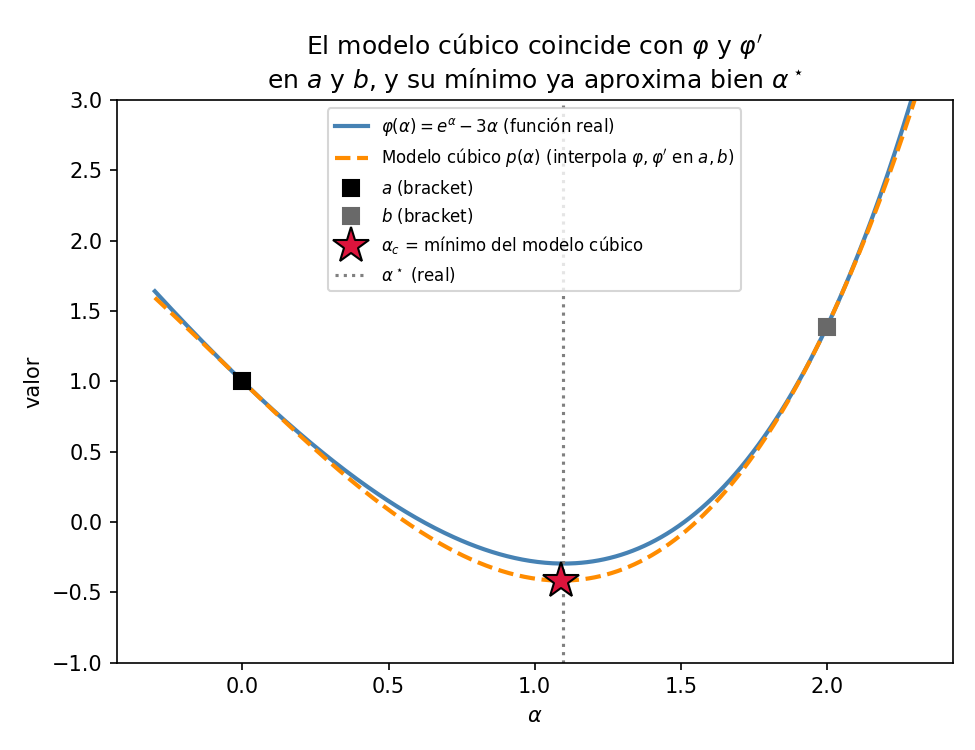
\includegraphics[height=0.82\textheight]{figs/fig00_cubico_modelo.png}
\end{frame}

\begin{frame}{Algoritmo: interpolaci\'on c\'ubica con bracket}
  An\'alogo a bisecci\'on, pero reemplazando el punto medio por el m\'inimo del modelo c\'ubico:
  \begin{enumerate}
    \item Partir de un bracket $[a,b]$ con $\varphi'(a)<0<\varphi'(b)$.
    \item Calcular $\alpha_c$ con la f\'ormula cerrada del c\'ubico.
    \item Evaluar $\varphi'(\alpha_c)$:
    \begin{itemize}
      \item si tiene el mismo signo que $\varphi'(a)$: $a \leftarrow \alpha_c$.
      \item si no: $b \leftarrow \alpha_c$.
    \end{itemize}
    \item Repetir hasta $|\varphi'(\alpha_c)| < \text{tol}$.
  \end{enumerate}
  \begin{alertblock}{Por qu\'e importa}
    Esta es, literalmente, la estrategia que usan internamente los line search \emph{serios} (condiciones de Wolfe) para refinar $\alpha$ una vez que se tiene un bracket: converge \textbf{superlinealmente}, muchas menos evaluaciones que bisecci\'on o b\'usqueda \'aurea.
  \end{alertblock}
\end{frame}

\begin{frame}[fragile]{C\'odigo: minimizaci\'on 1D por modelo c\'ubico}
\begin{lstlisting}
def cubic_step(a, b, phi, dphi):
    fa, fb = phi(a), phi(b);  ga, gb = dphi(a), dphi(b)
    d1 = ga + gb - 3.0 * (fa - fb) / (a - b)
    s = np.sign(b - a)
    d2 = s * np.sqrt(max(d1**2 - ga * gb, 0.0))
    return b - (b - a) * (gb + d2 - d1) / (gb - ga + 2 * d2)

def cubic_interpolation_1d(phi, dphi, a, b, tol=1e-10, max_iter=30):
    for _ in range(max_iter):
        alpha_c = cubic_step(a, b, phi, dphi)
        g_c = dphi(alpha_c)
        if abs(g_c) < tol:
            break
        if np.sign(g_c) == np.sign(dphi(a)):
            a = alpha_c
        else:
            b = alpha_c
    return alpha_c
\end{lstlisting}
\end{frame}

\begin{frame}{Ejemplo: $\varphi(\alpha)=e^\alpha-3\alpha$}
  M\'inimo exacto: $\varphi'(\alpha)=e^\alpha-3=0 \Rightarrow \alpha^\star=\ln 3 \approx 1.0986122887$. Bracket inicial $[0,2]$ ($\varphi'(0)=-2<0$, $\varphi'(2)=e^2-3>0$).
  \centering
  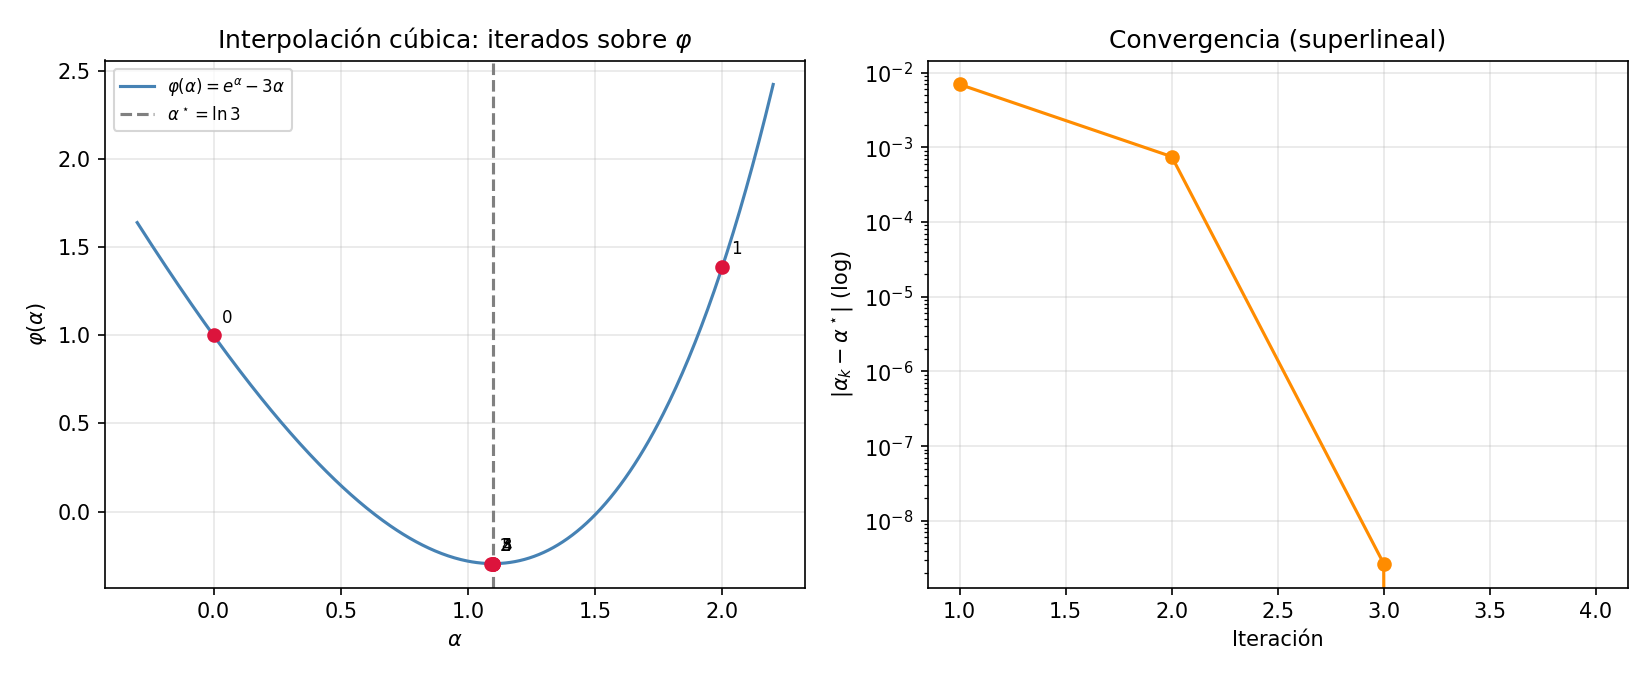
\includegraphics[height=0.68\textheight]{figs/fig00_cubico_1d.png}
\end{frame}

\begin{frame}{Resultados}
  \begin{itemize}
    \item \textbf{Interpolaci\'on c\'ubica}: \textbf{4} iteraciones, $\alpha_{\text{final}}=1.0986122887$ --- coincide con $\alpha^\star$ hasta precisi\'on de m\'aquina.
    \item \texttt{scipy.optimize.minimize\_scalar} (Brent, \textbf{sin} derivadas): 10 iteraciones para la misma precisi\'on.
  \end{itemize}
  \begin{alertblock}{La lecci\'on que llevamos al resto de la clase}
    Usar \textbf{derivadas} (aqu\'i, $\varphi'$; m\'as adelante, el gradiente completo $\grad f$ y hasta la Hessiana $H$) para construir un \textbf{modelo local} y minimizar ese modelo en vez de la funci\'on real, es la idea que atraviesa \emph{todos} los m\'etodos de esta clase --- del modelo lineal (descenso de gradiente) al cuadr\'atico (Newton, trust region) pasando por este modelo c\'ubico en 1D.
  \end{alertblock}
\end{frame}

% ============================================================
\section{Descenso de gradiente}
% ============================================================

\begin{frame}{Idea: el gradiente como direcci\'on de m\'aximo descenso}
  \small
  Del modelo lineal local de Taylor:
  \[ f(x_k + p) \approx f(x_k) + \grad f(x_k)^T p \]
  La direcci\'on $p$ (de norma fija) que \textbf{minimiza} este modelo lineal es
  \[ d_k = -\grad f(x_k) \]
  (recordar Clase 1: Cauchy-Schwarz $\Rightarrow$ $-\grad f$ es la direcci\'on de m\'aximo decrecimiento local).
  \begin{block}{Algoritmo: descenso de gradiente}
    \[ x_{k+1} = x_k - \alpha_k \, \grad f(x_k) \]
    Repetir hasta $\|\grad f(x_k)\| < \text{tol}$.
  \end{block}
  La pregunta clave: \textbf{\'c\'omo elegir $\alpha_k$}. Hoy vemos dos respuestas: paso fijo (ingenuo) y paso variable con line search (robusto).
\end{frame}

\begin{frame}[fragile]{C\'odigo: descenso de gradiente, paso fijo}
\begin{lstlisting}
def gradient_descent_fixed(f, grad, x0, alpha, n_iter=40):
    x = np.array(x0, dtype=float)
    traj = [x.copy()]
    for _ in range(n_iter):
        x = x - alpha * grad(x)
        traj.append(x.copy())
    return np.array(traj)
\end{lstlisting}
  \centering\small
  Extremadamente simple --- y extremadamente sensible a la elecci\'on de \texttt{alpha}, como veremos.
\end{frame}

\begin{frame}{Trayectoria: efecto del tama\~no de paso fijo}
  \centering
  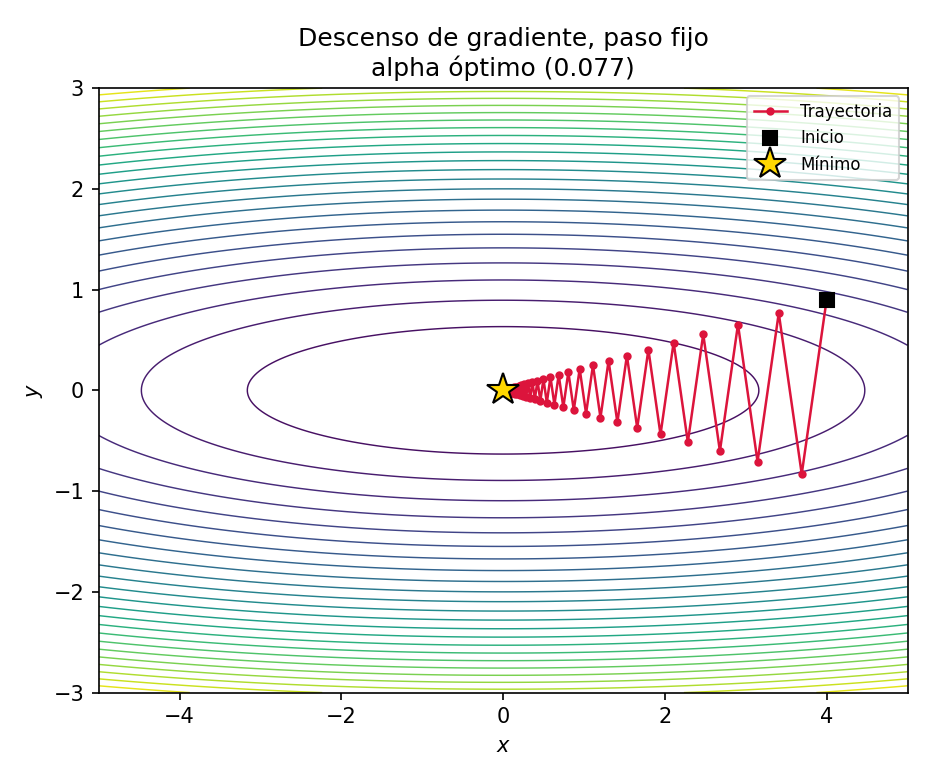
\includegraphics[height=0.82\textheight]{figs/fig01_gd_fijo_0.0769.png}
\end{frame}

\begin{frame}{Comparaci\'on: paso peque\~no vs. paso \'optimo vs. divergencia}
  \begin{columns}[T]
    \begin{column}{0.5\textwidth}
      \centering
      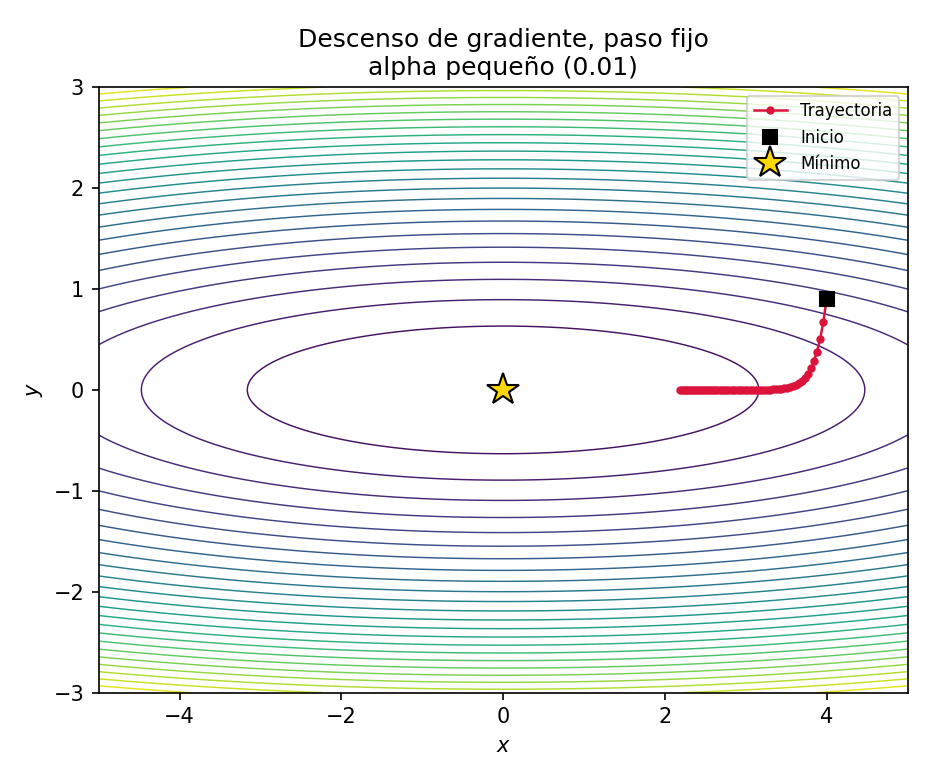
\includegraphics[width=0.92\textwidth]{figs/fig01_gd_fijo_0.0100.png}
    \end{column}
    \begin{column}{0.5\textwidth}
      \centering
      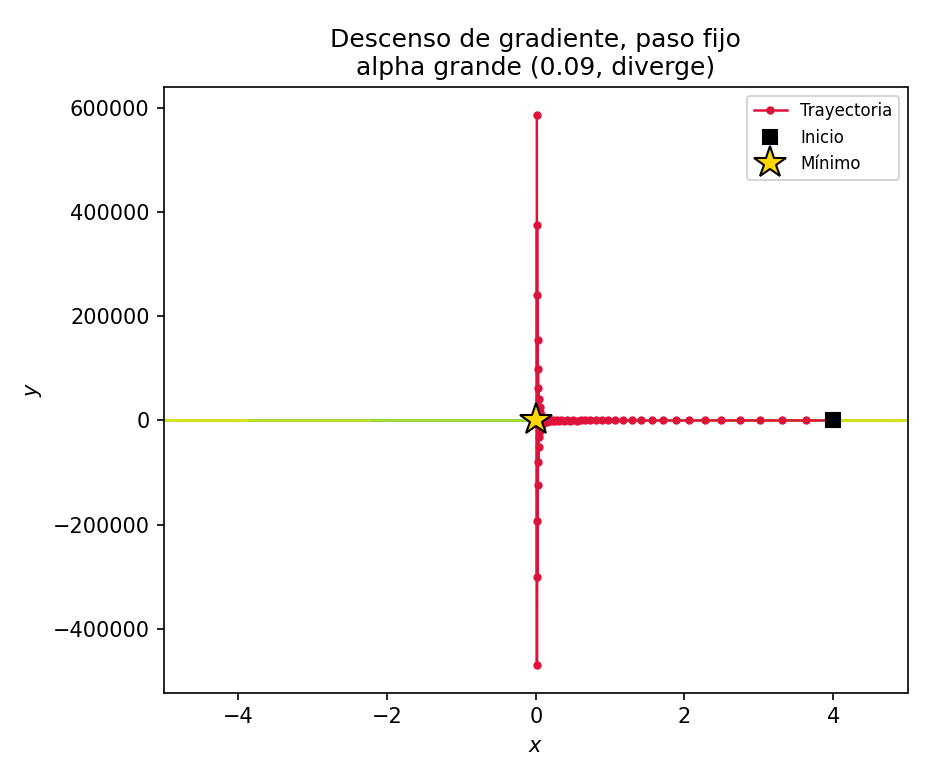
\includegraphics[width=0.92\textwidth]{figs/fig01_gd_fijo_0.0900.png}
    \end{column}
  \end{columns}
  \footnotesize
  \begin{itemize}
    \item Paso te\'orico \'optimo (autovalores $\{1,\kappa\}$): $\alpha^\star = 2/(1+\kappa)$.
    \item Con $\alpha > 2/\lambda_{\max}$ el m\'etodo \textbf{diverge}: $\alpha=0.09$ produce $f_{\text{final}} \approx 4\times10^{12}$ tras 60 iteraciones.
  \end{itemize}
\end{frame}

\begin{frame}{Convergencia: paso peque\~no vs. \'optimo}
  \centering
  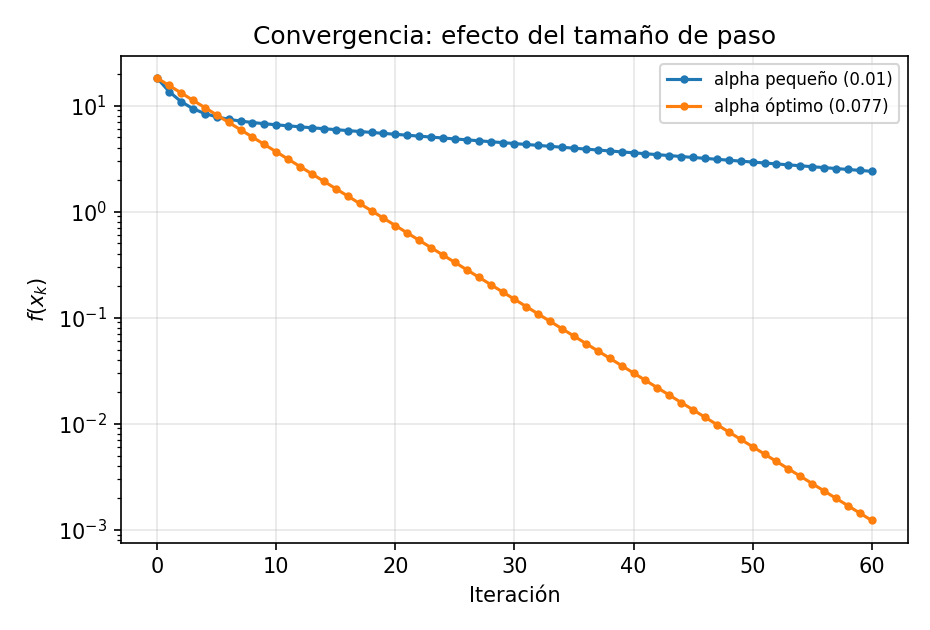
\includegraphics[height=0.82\textheight]{figs/fig01_gd_fijo_convergencia.png}
\end{frame}

\begin{frame}{El problema de fondo: elegir $\alpha$ a mano no escala}
  \begin{itemize}
    \item El paso \'optimo $\alpha^\star=2/(1+\kappa)$ solo existe en forma cerrada porque $f$ es \textbf{cuadr\'atica}. Para una $f$ general, no sabemos $\kappa$ de antemano.
    \item Un $\alpha$ fijo que funciona en una regi\'on de $f$ puede divergir en otra (curvatura variable).
    \item \textbf{Soluci\'on}: en lugar de fijar $\alpha$ a mano, calcularlo \emph{en cada iteraci\'on} resolviendo (aprox.) un problema de minimizaci\'on 1D. Eso es \textbf{line search} --- el tema que sigue.
  \end{itemize}
\end{frame}

% ============================================================
\section{Minimizaci\'on en una direcci\'on (line search)}
% ============================================================

\begin{frame}{Formalizaci\'on: la funci\'on de m\'erito $\varphi(\alpha)$}
  Dado $x_k$ y una direcci\'on de descenso $d_k$ (es decir, $\grad f(x_k)^T d_k < 0$), se define la funci\'on de una variable
  \[ \varphi(\alpha) = f(x_k + \alpha d_k), \qquad \alpha \geq 0 \]
  \textbf{Line search exacto}: resolver $\min_{\alpha \geq 0} \varphi(\alpha)$ (ej. con Brent 1D). Preciso, pero caro: requiere muchas evaluaciones de $f$ para un solo paso de $x_k$.

  \textbf{Line search inexacto}: en vez de minimizar $\varphi$ exactamente, aceptar el primer $\alpha$ que d\'e una reducci\'on ``suficiente''. Mucho m\'as barato y es lo que se usa en la pr\'actica.
\end{frame}

\begin{frame}{Condici\'on de Armijo (descenso suficiente)}
  \begin{block}{Condici\'on de Armijo}
    \[ \varphi(\alpha) \leq \varphi(0) + c_1\,\alpha\,\varphi'(0), \qquad c_1 \in (0,1) \text{ (t\'ipicamente } c_1=10^{-4}\text{)} \]
  \end{block}
  Geom\'etricamente: la recta $\varphi(0)+c_1\alpha\varphi'(0)$ tiene la pendiente inicial de $\varphi$ ``achicada'' por $c_1$; cualquier $\alpha$ cuya $\varphi(\alpha)$ quede \textbf{por debajo} de esa recta se acepta.

  \begin{block}{Backtracking (algoritmo pr\'actico)}
    \begin{enumerate}
      \item Empezar con $\alpha = \alpha_0$ (ej. $\alpha_0=1$).
      \item Si se cumple Armijo, aceptar $\alpha$ y terminar.
      \item Si no, $\alpha \leftarrow \rho\,\alpha$ (ej. $\rho=0.5$) y volver a 2.
    \end{enumerate}
  \end{block}
\end{frame}

\begin{frame}[fragile]{C\'odigo: backtracking Armijo}
\begin{lstlisting}
def armijo_backtracking(f, grad, x, d, alpha0=1.0, c1=1e-4, rho=0.5):
    phi0 = f(x)
    dphi0 = grad(x) @ d
    alpha = alpha0
    while f(x + alpha * d) > phi0 + c1 * alpha * dphi0:
        alpha *= rho
    return alpha
\end{lstlisting}
\end{frame}

\begin{frame}{Visualizaci\'on: $\varphi(\alpha)$, l\'imite de Armijo y backtracking}
  \centering
  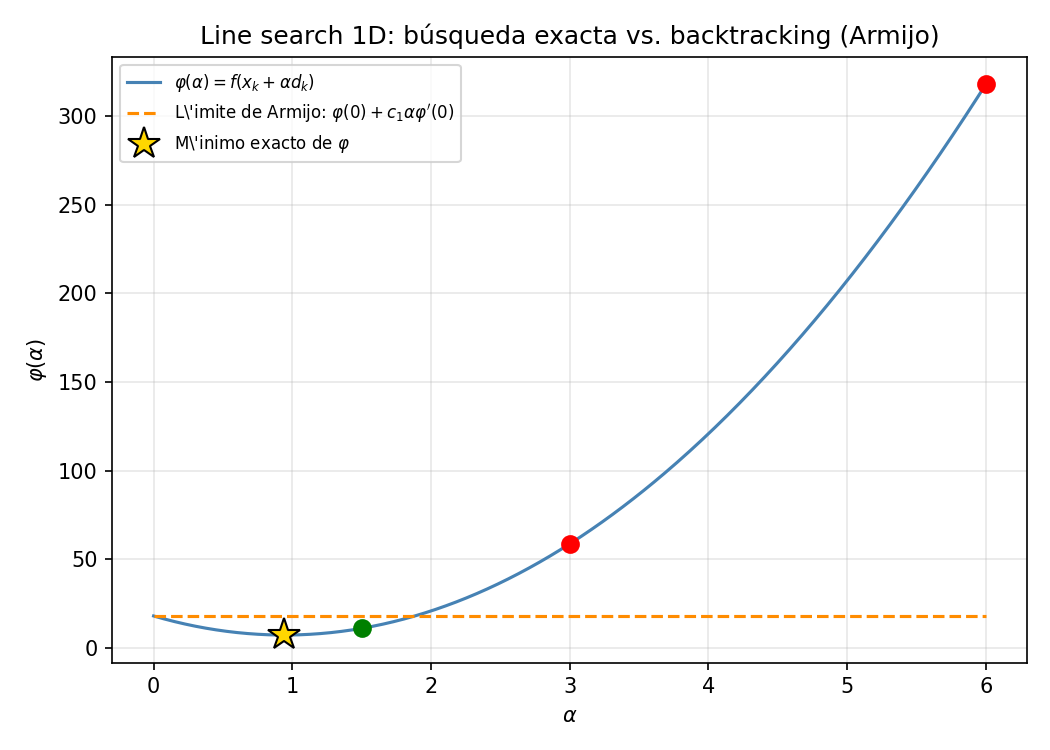
\includegraphics[height=0.82\textheight]{figs/fig02_line_search_phi.png}
\end{frame}

\begin{frame}{Lectura de la figura}
  \begin{itemize}
    \item El m\'inimo \textbf{exacto} de $\varphi$ (estrella dorada) est\'a en $\alpha^\star \approx 0.94$.
    \item Backtracking arranca en $\alpha_0=6$ y prueba $6 \to 3 \to 1.5$: los dos primeros se \textbf{rechazan} (quedan por encima de la recta l\'imite de Armijo), el tercero se \textbf{acepta}.
    \item El $\alpha$ aceptado por Armijo (1.5) no es el m\'inimo exacto de $\varphi$ --- y no hace falta que lo sea: solo se pide una reducci\'on suficiente, mucho m\'as barato de verificar.
  \end{itemize}
  \begin{alertblock}{Nota}
    En la pr\'actica se suele combinar Armijo con una segunda condici\'on (curvatura, condiciones de Wolfe) para evitar pasos demasiado cortos. Aqu\'i usamos solo Armijo + backtracking por simplicidad, suficiente para garantizar convergencia global junto con descenso de gradiente.
  \end{alertblock}
\end{frame}

% ============================================================
\section{Descenso de gradiente con convergencia global}
% ============================================================

\begin{frame}{Combinando gradiente + line search}
  \begin{block}{Algoritmo: descenso de gradiente con paso variable}
    \begin{enumerate}
      \item $d_k = -\grad f(x_k)$
      \item $\alpha_k = $ backtracking Armijo a lo largo de $d_k$ (line search 1D)
      \item $x_{k+1} = x_k + \alpha_k d_k$
      \item Repetir hasta $\|\grad f(x_k)\| < $ tol
    \end{enumerate}
  \end{block}
  \begin{alertblock}{\emph{Convergencia global} --- precisi\'on de lenguaje}
    Significa que el m\'etodo converge a un punto \textbf{estacionario} desde \emph{cualquier} punto inicial --- NO que encuentre el m\'inimo global de una funci\'on no convexa. Es terminolog\'ia est\'andar (Nocedal \& Wright, cap.\ 3), distinta de \emph{\'optimo global}.
  \end{alertblock}
  A diferencia del paso fijo (script anterior), este m\'etodo \textbf{nunca diverge}: Armijo garantiza que cada paso efectivamente reduce $f$.
\end{frame}

\begin{frame}{Trayectoria en Rosenbrock}
  \centering
  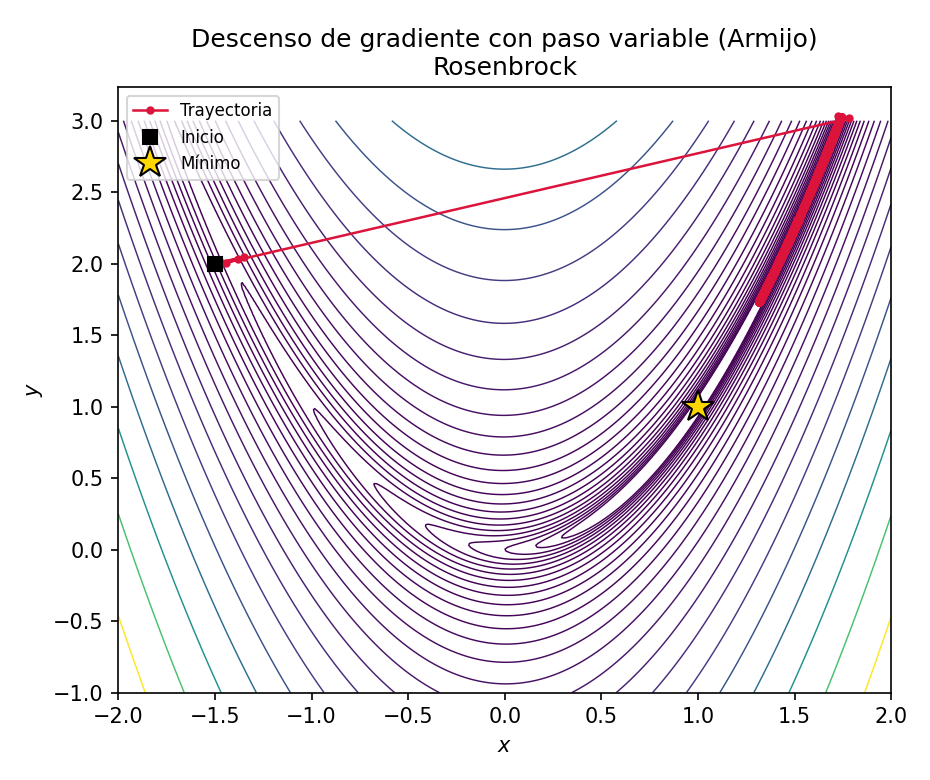
\includegraphics[height=0.82\textheight]{figs/fig03_gd_armijo_rosenbrock.png}
\end{frame}

\begin{frame}{Convergencia --- y su costo}
  \begin{columns}[T]
    \begin{column}{0.55\textwidth}
      \centering
      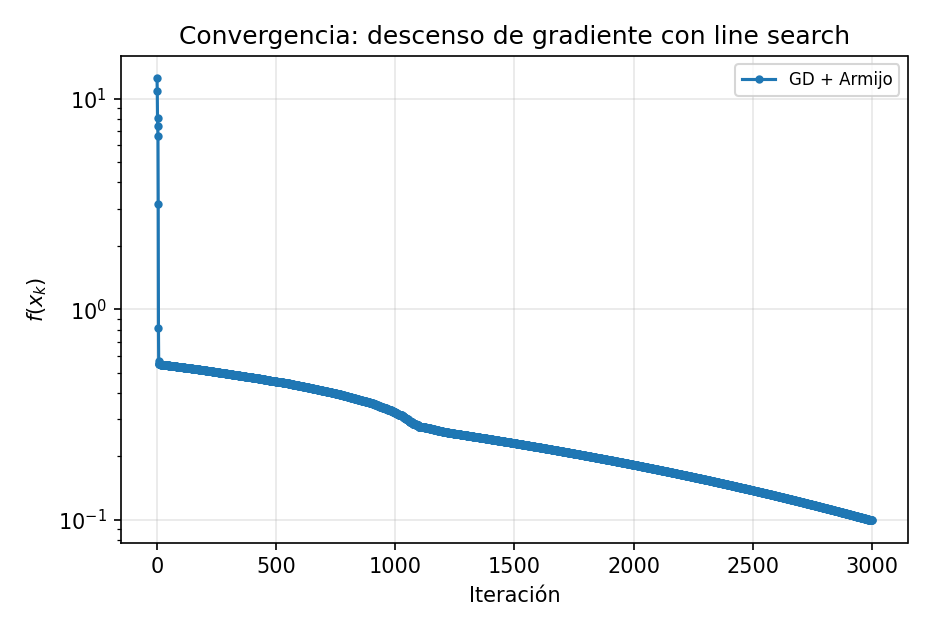
\includegraphics[width=\textwidth]{figs/fig03_gd_armijo_convergencia.png}
    \end{column}
    \begin{column}{0.43\textwidth}
      \small
      \begin{itemize}
        \item GD + Armijo: \textbf{no converge del todo} en 3000 iter.\ ($f\approx0.099$).
        \item \texttt{scipy CG} (Wolfe): converge en solo \textbf{29} iter.
      \end{itemize}
      \begin{alertblock}{\small Punto pedag\'ogico}
        \small Robusto $\neq$ r\'apido. El valle curvo de Rosenbrock es el peor caso para descenso de gradiente puro. Motiva usar \textbf{curvatura} (Newton/quasi-Newton).
      \end{alertblock}
    \end{column}
  \end{columns}
\end{frame}
% ============================================================
\section{M\'etodo de Powell}
% ============================================================

\begin{frame}{Motivaci\'on: optimizaci\'on sin gradiente}
  \begin{itemize}
    \item Todos los m\'etodos anteriores necesitan $\grad f$ (anal\'itico o autom\'atico).
    \item ?`Qu\'e hacer si $f$ es una caja negra (ej. una simulaci\'on costosa) sin gradiente disponible?
    \item \textbf{Powell (1964)}: minimiza sucesivamente a lo largo de \textbf{direcciones}, usando solo evaluaciones de $f$ (line search 1D repetido), y construye \textbf{direcciones conjugadas} sobre la marcha para acelerar la convergencia respecto a usar siempre los ejes coordenados.
  \end{itemize}
  \begin{block}{Direcciones conjugadas (recordatorio, cuadr\'aticas)}
    Dos direcciones $d_i, d_j$ son conjugadas respecto a $H$ si $d_i^T H d_j = 0$. Minimizar sucesivamente a lo largo de $n$ direcciones conjugadas resuelve una cuadr\'atica $n$-dimensional \textbf{exactamente} en $n$ pasos --- mucho mejor que los ejes coordenados, que hacen zig-zag igual que el descenso de gradiente.
  \end{block}
\end{frame}

\begin{frame}{Algoritmo de Powell (un ciclo, $n=2$)}
  Direcciones iniciales: $d_1=e_1=(1,0)$, $d_2=e_2=(0,1)$.
  \begin{enumerate}
    \item Desde $x_0$: line search exacto a lo largo de $d_1$ $\to x_1$.
    \item Desde $x_1$: line search exacto a lo largo de $d_2$ $\to x_2$.
    \item Nueva direcci\'on conjugada: $d_{\text{new}} = x_2 - x_0$.
    \item Line search a lo largo de $d_{\text{new}}$ desde $x_2$ $\to x_3$.
    \item \textbf{Regla de Powell}: descartar la direcci\'on que m\'as redujo $f$ en este ciclo, reemplazarla por $d_{\text{new}}$.
    \item Repetir el ciclo con el conjunto de direcciones actualizado.
  \end{enumerate}
  \begin{alertblock}{Salvaguarda usada en el c\'odigo}
    En valles muy curvos (Rosenbrock), un line search 1D puede no ser unimodal en el rango buscado. Se agrega la salvaguarda: si el resultado es peor que no moverse, se conserva el punto de partida.
  \end{alertblock}
\end{frame}

\begin{frame}[fragile]{C\'odigo: n\'ucleo del m\'etodo de Powell}
\begin{lstlisting}
def line_search_along(f, x, d, bracket=(-2, 2)):
    def phi(alpha):
        return f(x + alpha * d)
    res = minimize_scalar(phi, bracket=bracket)
    if res.fun <= phi(0.0):
        return x + res.x * d, res.fun
    return x.copy(), phi(0.0)   # salvaguarda

# ciclo: line search a lo largo de cada direccion,
# luego direccion conjugada d_new = x_final - x_inicial,
# reemplazar la direccion que mas redujo f por d_new
\end{lstlisting}
\end{frame}

\begin{frame}{Trayectoria: Powell en Rosenbrock}
  \centering
  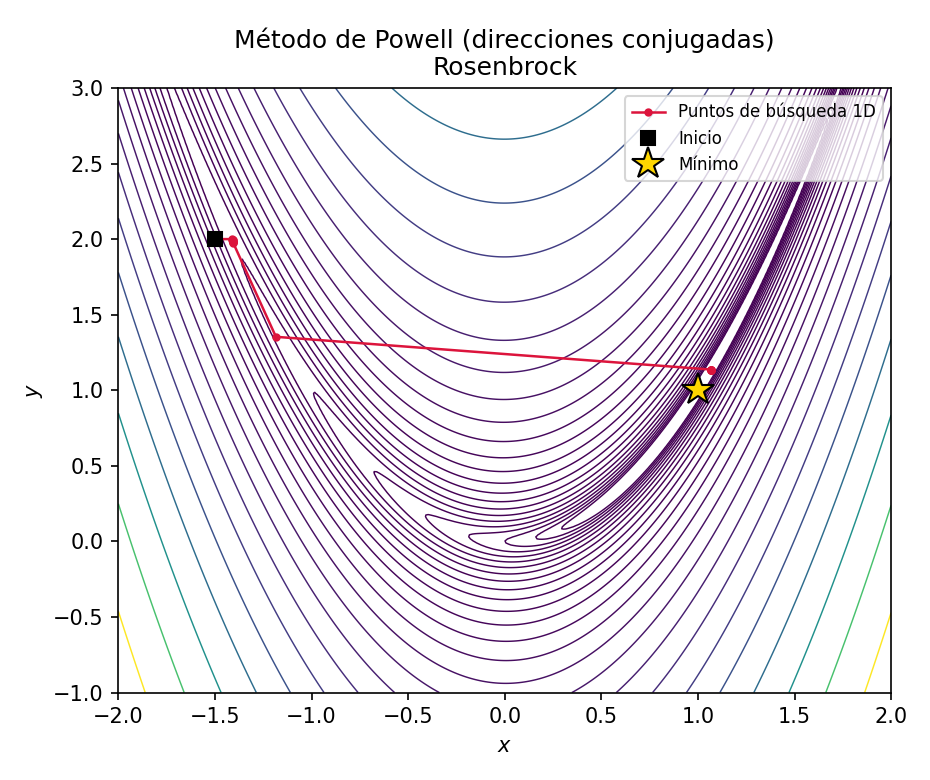
\includegraphics[height=0.82\textheight]{figs/fig04_powell_rosenbrock.png}
\end{frame}

\begin{frame}{Resultados y comparaci\'on con \texttt{scipy}}
  \begin{itemize}
    \item \textbf{Powell manual}: 5 ciclos (15 line searches 1D), $f_{\text{final}} \approx 4.4\times10^{-3}$.
    \item \textbf{\texttt{scipy.optimize.minimize(method=`Powell')}}: 25 iteraciones, 670 evaluaciones de $f$, $f_{\text{final}} \approx 2.7\times10^{-29}$ (esencialmente exacto).
  \end{itemize}
  \begin{alertblock}{Por qu\'e la diferencia}
    La implementaci\'on de \texttt{scipy} incluye salvaguardas adicionales (verificaci\'on de que las direcciones no se vuelvan casi paralelas/linealmente dependientes, reinicios peri\'odicos a los ejes coordenados) que nuestra versi\'on did\'actica omite por claridad. El mecanismo de fondo --- direcciones conjugadas construidas sin gradiente --- es el mismo.
  \end{alertblock}
\end{frame}
% ============================================================
\section{M\'etodo de Newton}
% ============================================================

\begin{frame}{Del modelo lineal al modelo cuadr\'atico}
  Descenso de gradiente usa el modelo \textbf{lineal} de Taylor. El m\'etodo de Newton usa el modelo \textbf{cuadr\'atico} (Clase 1, serie de Taylor de 2do orden):
  \[ m_k(p) = f(x_k) + \grad f(x_k)^T p + \tfrac12\, p^T H(x_k)\, p \]
  Minimizando $m_k$ respecto a $p$ (asumiendo $H(x_k)$ definida positiva):
  \[ \grad_p m_k(p) = \grad f(x_k) + H(x_k)\, p = 0 \;\;\Longrightarrow\;\; p_k = -H(x_k)^{-1}\, \grad f(x_k) \]
  \begin{block}{Paso de Newton puro}
    \[ x_{k+1} = x_k + p_k \qquad (\alpha_k = 1 \text{ fijo}) \]
  \end{block}
  En una cuadr\'atica exacta, el modelo $m_k$ coincide con $f$ $\Rightarrow$ \textbf{un solo paso} basta.
\end{frame}

\begin{frame}{Trayectoria: Newton puro en la cuadr\'atica}
  \centering
  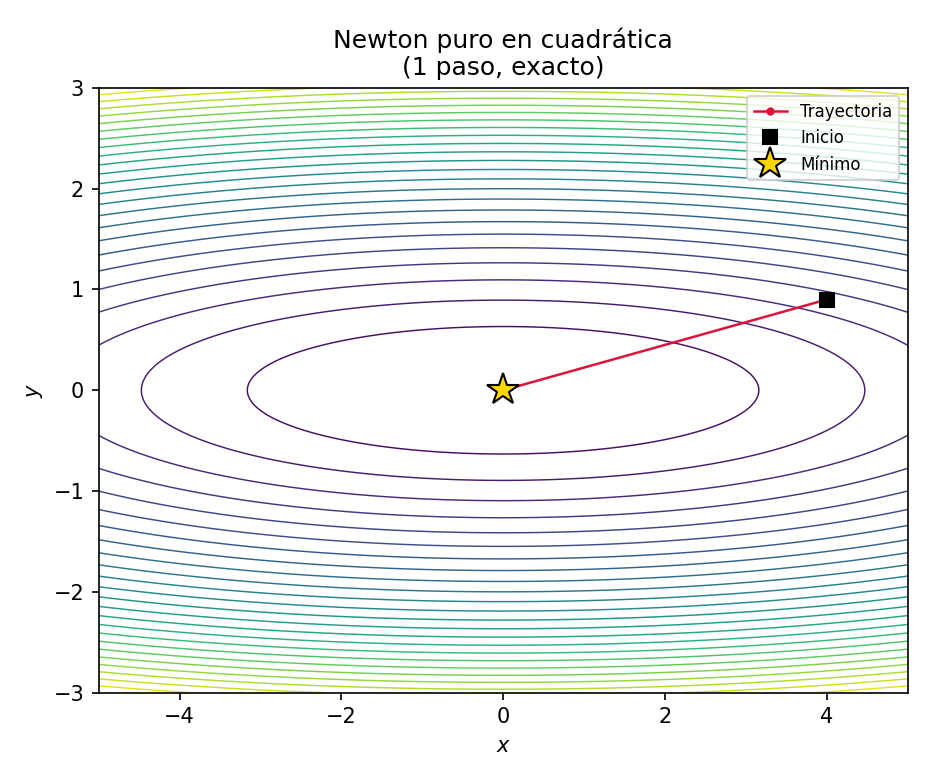
\includegraphics[height=0.82\textheight]{figs/fig05_newton_cuadratica.png}
\end{frame}

\begin{frame}{Newton en funciones no cuadr\'aticas: convergencia y riesgos}
  \begin{itemize}
    \item Para $f$ general, $m_k$ solo aproxima a $f$ localmente $\Rightarrow$ Newton necesita varias iteraciones, pero converge con \textbf{orden cuadr\'atico} cerca del m\'inimo (el n\'umero de d\'igitos correctos se duplica en cada paso).
    \item \textbf{Riesgo}: si $H(x_k)$ no es definida positiva (lejos del m\'inimo, en zonas de curvatura mixta), $p_k$ puede no ser direcci\'on de descenso, o incluso apuntar hacia un m\'aximo/silla.
  \end{itemize}
  \begin{block}{Newton amortiguado (\emph{damped Newton})}
    Salvaguarda pr\'actica:
    \begin{enumerate}
      \item Si $\grad f(x_k)^T p_k \geq 0$ (no es descenso), usar $p_k=-\grad f(x_k)$ en su lugar.
      \item Aplicar backtracking Armijo sobre $\alpha$ (en vez de $\alpha=1$ fijo).
    \end{enumerate}
    As\'i se preserva la velocidad de Newton cerca del \'optimo, con la robustez de line search lejos de \'el.
  \end{block}
\end{frame}

\begin{frame}[fragile]{C\'odigo: Newton amortiguado}
\begin{lstlisting}
g = grad(x); H = hess(x)
p = np.linalg.solve(H, -g)          # paso de Newton
if g @ p >= 0:                       # salvaguarda: no es descenso
    p = -g
alpha = 1.0
while f(x + alpha*p) > f(x) + 1e-4*alpha*(g @ p):
    alpha *= 0.5                     # backtracking Armijo
x = x + alpha * p
\end{lstlisting}
\end{frame}

\begin{frame}{Trayectoria: Newton amortiguado en Rosenbrock}
  \centering
  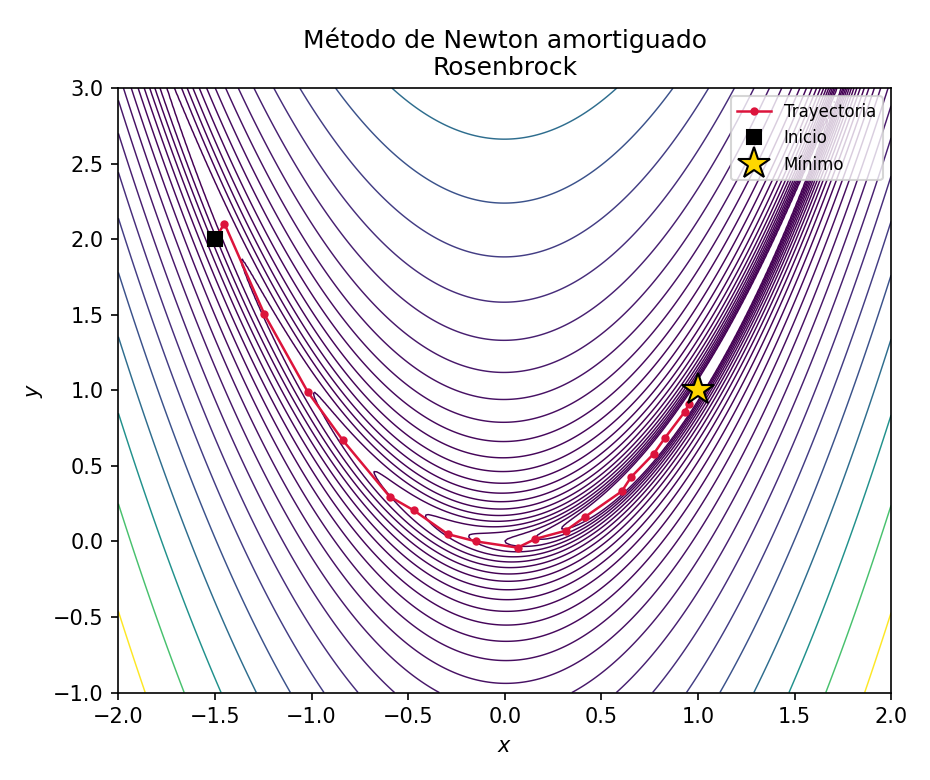
\includegraphics[height=0.82\textheight]{figs/fig05_newton_rosenbrock.png}
\end{frame}

\begin{frame}{Resultados: velocidad de Newton}
  \centering
  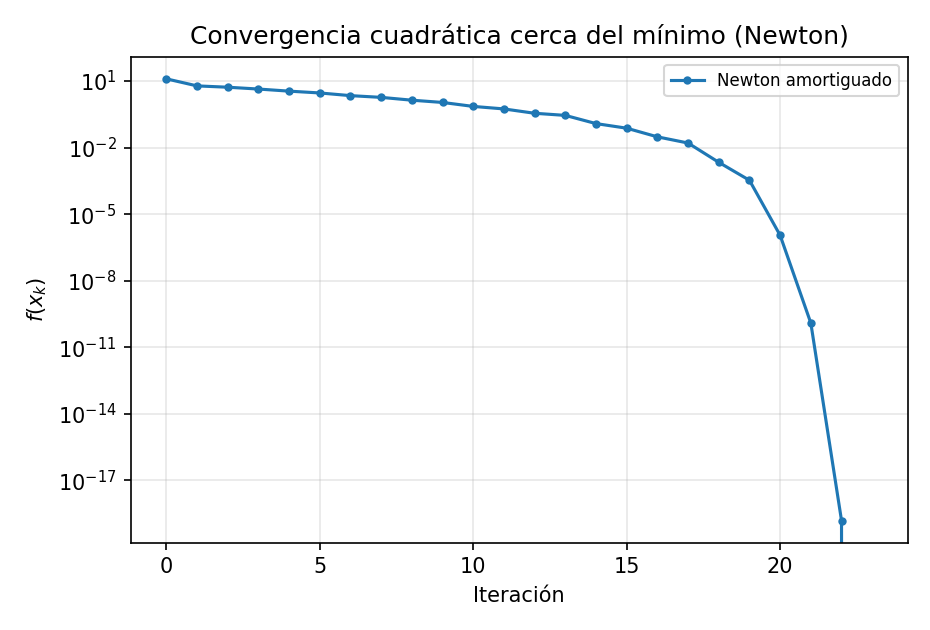
\includegraphics[height=0.55\textheight]{figs/fig05_newton_convergencia.png}
  \begin{itemize}
    \small
    \item Newton amortiguado: \textbf{24} iteraciones hasta $f\approx0$.
    \item \texttt{scipy Newton-CG}: 191 iteraciones (usa un solver iterativo --gradiente conjugado-- para el sistema lineal, en vez de resolverlo exactamente como aqu\'i).
    \item Comparar con descenso de gradiente + Armijo: \textbf{3000} iteraciones sin convergencia completa (script anterior). La curvatura (Hessiana) es lo que marca la diferencia.
  \end{itemize}
\end{frame}

% ============================================================
\section{Newton con Hessiana aproximada (quasi-Newton, BFGS)}
% ============================================================

\begin{frame}{Motivaci\'on}
  \begin{itemize}
    \item Newton exacto necesita calcular \textbf{y factorizar} $H(x_k)$ en cada iteraci\'on: costoso ($O(n^3)$ para factorizar, $O(n^2)$ para almacenar), y a veces $H$ ni siquiera est\'a disponible anal\'iticamente.
    \item \textbf{Idea quasi-Newton}: construir una \textbf{aproximaci\'on} $B_k \approx H(x_k)$ (o directamente de su inversa) usando solo informaci\'on de \textbf{gradientes} ya calculados --- sin nunca evaluar la Hessiana real.
  \end{itemize}
  \begin{block}{BFGS (Broyden--Fletcher--Goldfarb--Shanno)}
    Con $s_k = x_{k+1}-x_k$ y $y_k = \grad f(x_{k+1}) - \grad f(x_k)$:
    \[
    H_{k+1}^{-1} = (I-\rho_k s_k y_k^T)\, H_k^{-1}\, (I-\rho_k y_k s_k^T) + \rho_k s_k s_k^T,
    \quad \rho_k = \frac{1}{y_k^T s_k}
    \]
  \end{block}
\end{frame}

\begin{frame}{Propiedades clave de BFGS}
  \begin{itemize}
    \item Se inicializa $H_0^{-1}=I$ (el primer paso equivale a descenso de gradiente).
    \item Cada iteraci\'on: $p_k = -H_k^{-1}\grad f(x_k)$, luego line search (Armijo) en esa direcci\'on.
    \item \textbf{Condici\'on de curvatura}: si $y_k^T s_k > 0$, la actualizaci\'on preserva autom\'aticamente que $H_k^{-1}$ sea definida positiva $\Rightarrow$ $p_k$ \textbf{siempre} es direcci\'on de descenso (a diferencia de Newton puro, no hace falta verificar autovalores).
    \item Convergencia \textbf{superlineal} (m\'as lenta que la cuadr\'atica de Newton, pero sin necesitar la Hessiana real).
  \end{itemize}
\end{frame}

\begin{frame}[fragile]{C\'odigo: actualizaci\'on BFGS}
\begin{lstlisting}
s = x_new - x;  y = g_new - g
sy = y @ s
if sy > 1e-12:                       # condicion de curvatura
    rho = 1.0 / sy
    V = np.eye(n) - rho * np.outer(s, y)
    Hinv = V @ Hinv @ V.T + rho * np.outer(s, s)
# si sy <= 0, se conserva Hinv (salvaguarda)
\end{lstlisting}
\end{frame}

\begin{frame}{Trayectoria: BFGS en Rosenbrock}
  \centering
  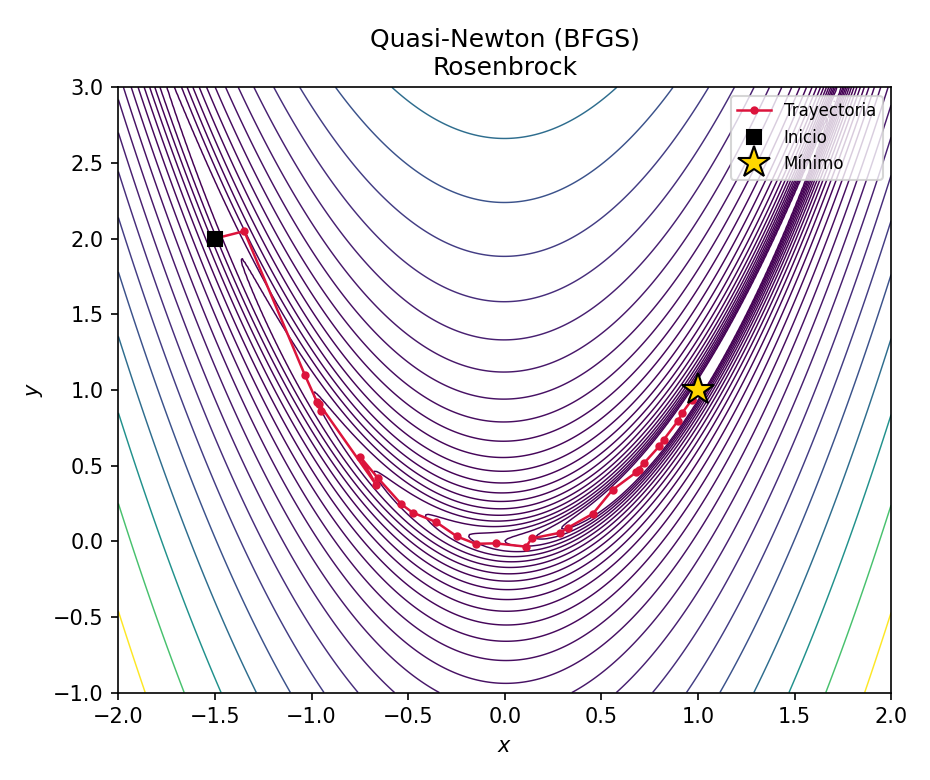
\includegraphics[height=0.82\textheight]{figs/fig06_bfgs_rosenbrock.png}
\end{frame}

\begin{frame}{Resultados}
  \centering
  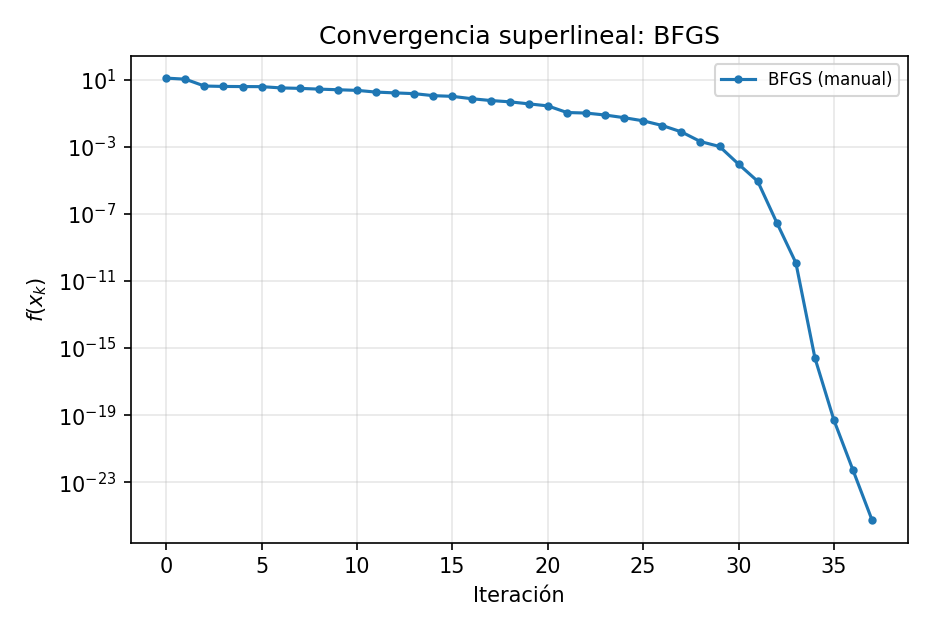
\includegraphics[height=0.5\textheight]{figs/fig06_bfgs_convergencia.png}
  \begin{itemize}
    \small
    \item BFGS manual: \textbf{38} iteraciones, $f_{\text{final}}\approx5\times10^{-26}$.
    \item \texttt{scipy.optimize.minimize(method=`BFGS')}: 37 iteraciones --- pr\'acticamente id\'entico.
    \item Tabla comparativa (misma Rosenbrock, mismo punto inicial): Newton exacto 24 iter, BFGS 38 iter, descenso de gradiente+Armijo no converge en 3000.
  \end{itemize}
\end{frame}
% ============================================================
\section{Trust region: m\'etodo dogleg}
% ============================================================

\begin{frame}{Trust region: otra forma de usar el modelo cuadr\'atico}
  Recordar el modelo cuadr\'atico local:
  \[ m_k(p) = f(x_k) + \grad f(x_k)^T p + \tfrac12\, p^T H_k\, p \]
  \textbf{Line search} (Newton, BFGS): confiar en $m_k$ en \emph{toda} una direcci\'on, y ajustar solo cu\'anto avanzar.

  \textbf{Trust region}: reconocer que $m_k$ solo es confiable \textbf{cerca} de $x_k$, y resolver:
  \[ \min_{p} \; m_k(p) \qquad \text{sujeto a} \qquad \|p\| \leq \Delta_k \]
  Esto decide \textbf{direcci\'on y magnitud del paso simult\'aneamente}, dentro de una bola de radio $\Delta_k$ (la ``regi\'on de confianza'').

  \begin{alertblock}{El subproblema exacto es caro}
    Resolver el subproblema restringido \emph{exactamente} requiere \'algebra no trivial. El m\'etodo \textbf{dogleg} lo aproxima de forma barata y muy efectiva.
  \end{alertblock}
\end{frame}

\begin{frame}{Trust region en 1D: el subproblema se resuelve a mano}
  \small
  Una variable: el modelo es una par\'abola y la regi\'on de confianza es un \textbf{intervalo}, con $g=f'(x_k)$, $h=f''(x_k)$:
  \[ \min_{p}\; m_k(p) = f(x_k) + g\,p + \tfrac12\, h\, p^2 \quad \text{s.a.} \quad |p| \leq \Delta_k \]
  El t\'ermino constante $f(x_k)$ no cambia d\'onde est\'a el m\'inimo, pero s\'i es parte del modelo (la par\'abola naranja de las figuras pasa por $(x_k,f(x_k))$).
  \begin{block}{Tres casos}
    \begin{enumerate}
      \item $h>0$ y $|g/h|\leq\Delta_k$: el m\'inimo de la par\'abola cabe $\Rightarrow$ \textbf{paso de Newton}, $p=-g/h$.
      \item $h>0$ y $|g/h|>\Delta_k$: queda fuera $\Rightarrow$ \textbf{al borde}, $p=-\mathrm{sgn}(g)\,\Delta_k$.
      \item $h\leq0$ (curvatura negativa o nula): no hay m\'inimo $\Rightarrow$ \textbf{al borde} cuesta abajo, $p=-\mathrm{sgn}(g)\,\Delta_k$.
    \end{enumerate}
  \end{block}
\end{frame}

\begin{frame}{?`Y el paso de Cauchy y el dogleg en 1D?}
  \begin{itemize}
    \item En 1D, $-g$ (direcci\'on de Cauchy) y $-g/h$ (direcci\'on de Newton) apuntan \textbf{al mismo lado}: son \textbf{colineales}.
    \item Por eso la poligonal dogleg se reduce a un segmento recto, y el paso es simplemente \emph{Newton recortado a la regi\'on de confianza}.
  \end{itemize}
  \begin{alertblock}{Lo que s\'i se ve igual que en varias variables}
    El papel de la regi\'on de confianza (limitar el paso), el manejo de curvatura negativa (ir al borde) y la regla de aceptaci\'on y de radio con $\rho_k$. En 2D o m\'as, Cauchy y Newton apuntan en direcciones distintas, y ah\'i s\'i hace falta combinarlos: es el dogleg de las siguientes diapositivas.
  \end{alertblock}
\end{frame}

\begin{frame}{?`Se acepta el paso? El ratio $\rho_k$ y el radio}
  \small
  El modelo puede equivocarse lejos de $x_k$. Se compara lo que \textbf{predijo} contra lo que \textbf{pas\'o}:
  \[ \rho_k = \frac{f(x_k)-f(x_k+p_k)}{m_k(0)-m_k(p_k)} = \frac{\text{reducci\'on real}}{\text{reducci\'on predicha}} \]
  \begin{columns}[T]
    \begin{column}{0.48\textwidth}
      \begin{block}{Aceptar o rechazar}
        \begin{itemize}
          \item $\rho_k>0$: $f$ baj\'o $\Rightarrow$ se \textbf{acepta} $x_{k+1}=x_k+p_k$.
          \item $\rho_k\leq0$: $f$ no baj\'o $\Rightarrow$ se \textbf{rechaza}, $x_{k+1}=x_k$.
        \end{itemize}
      \end{block}
    \end{column}
    \begin{column}{0.48\textwidth}
      \begin{block}{Qu\'e hacer con $\Delta_k$}
        \begin{itemize}
          \item $\rho_k<1/4$: \textbf{encoger}, $\Delta/4$.
          \item $\rho_k>3/4$ y $|p_k|=\Delta_k$: \textbf{crecer}, $2\Delta$.
          \item en otro caso: \textbf{mantener}.
        \end{itemize}
      \end{block}
    \end{column}
  \end{columns}
  \vspace{0.2cm}
  Es exactamente la misma regla que se usa en dogleg y Levenberg-Marquardt; en 1D se puede ver paso a paso.
\end{frame}

\begin{frame}{?`Por qu\'e basta $\rho_k>0$?}
  \small
  Un cociente de dos negativos tambi\'en es positivo: ?`se aceptar\'ia un paso donde $f$ y el modelo \emph{suben}?
  \begin{block}{No: el denominador nunca es negativo}
    $p=0$ es factible y el paso minimiza (aprox.) el modelo en la regi\'on, as\'i que $m_k(p)\leq m_k(0)$:
    \[ m_k(0)-m_k(p) \;\geq\; 0 \qquad (\text{y } >0 \text{ si } g\neq0) \]
    Por tanto $\rho_k$ tiene el signo de la reducci\'on \textbf{real}: $\rho_k>0 \iff f$ baj\'o.
  \end{block}
  \footnotesize
  Verificaci\'on en 1D, con $\text{pred}=-(g\,p+\tfrac12 h\,p^2)$:
  \centering
  \begin{tabular}{lcc}
    \toprule
    Caso & Paso $p$ & Reducci\'on predicha \\
    \midrule
    $h>0$, Newton cabe & $-g/h$ & $\dfrac{g^2}{2h}>0$ \\[2pt]
    $h>0$, $|g/h|>\Delta_k$ & $-\mathrm{sgn}(g)\Delta_k$ & $\Delta_k\big(|g|-\tfrac12 h\Delta_k\big)>\tfrac12|g|\Delta_k>0$ \\[2pt]
    $h\leq0$ & $-\mathrm{sgn}(g)\Delta_k$ & $|g|\Delta_k-\tfrac12 h\Delta_k^2\geq|g|\Delta_k>0$ \\
    \bottomrule
  \end{tabular}
\end{frame}

\begin{frame}{La garant\'ia en varias variables (y cu\'ando falla)}
  \small
  \begin{block}{Condici\'on de descenso de Cauchy}
    Todo paso aceptable debe reducir el modelo al menos tanto como el punto de Cauchy:
    \[ m_k(0)-m_k(p_k) \;\geq\; \tfrac12\,\|\grad f_k\|\,\min\!\Big(\Delta_k,\ \frac{\|\grad f_k\|}{\|H_k\|}\Big) > 0 \]
    Cauchy la cumple siempre. El dogleg la cumple si $H_k$ es \textbf{definida positiva}: el modelo decrece a lo largo de la poligonal (Nocedal \& Wright, Lema 4.2).
  \end{block}
  \begin{alertblock}{Si $H_k$ no es definida positiva}
    $p_N$ ya no minimiza el modelo (puede ser un punto silla) y este puede \emph{subir}. Ejemplo: $g=(1,1)$, $H=\mathrm{diag}(-1,2)$, $\Delta=10$ da $m(0)-m(p_N)=-0.25<0$. Por eso el c\'odigo usa \textbf{solo Cauchy} si $H_k$ no es definida positiva.
  \end{alertblock}
  \texttt{rho = actual/pred if pred > 1e-14 else -1.0} tambi\'en cubre $\text{pred}\approx0$ (ya en el m\'inimo): no se divide y se rechaza.
\end{frame}

\begin{frame}[fragile]{C\'odigo: trust region en 1D}
\begin{lstlisting}
def tr_step_1d(g, h, Delta):
    if h > 0 and abs(g / h) <= Delta:
        return -g / h                    # caso 1: Newton cabe
    return -np.sign(g) * Delta           # casos 2 y 3: al borde
while abs(df(x)) > tol:
    g, h = df(x), d2f(x)
    p = tr_step_1d(g, h, Delta)
    pred   = -(g * p + 0.5 * h * p**2)   # m(0) - m(p)
    actual = f(x) - f(x + p)
    rho = actual / pred if pred > 1e-14 else -1.0
    if rho < 0.25:
        Delta = 0.25 * Delta                     # encoger
    elif rho > 0.75 and np.isclose(abs(p), Delta):
        Delta = min(2 * Delta, Delta_max)        # crecer
    if rho > 0:
        x = x + p                        # aceptar; si no, x no cambia
\end{lstlisting}
\end{frame}

\begin{frame}{Ejemplo: $f(x)=x^4-4x^2+x$, partiendo de $x_0=0.4$, $\Delta_0=0.5$}
  \small
  Dos m\'inimos locales (en $\approx-1.47$ y $\approx1.35$) y un m\'aximo local cerca de $x\approx0.13$. En $x_0=0.4$: $f''(x_0)=-6.08<0$, \textbf{curvatura negativa}: Newton puro ir\'ia hacia el m\'aximo.
  \vspace{0.2cm}
  \centering
  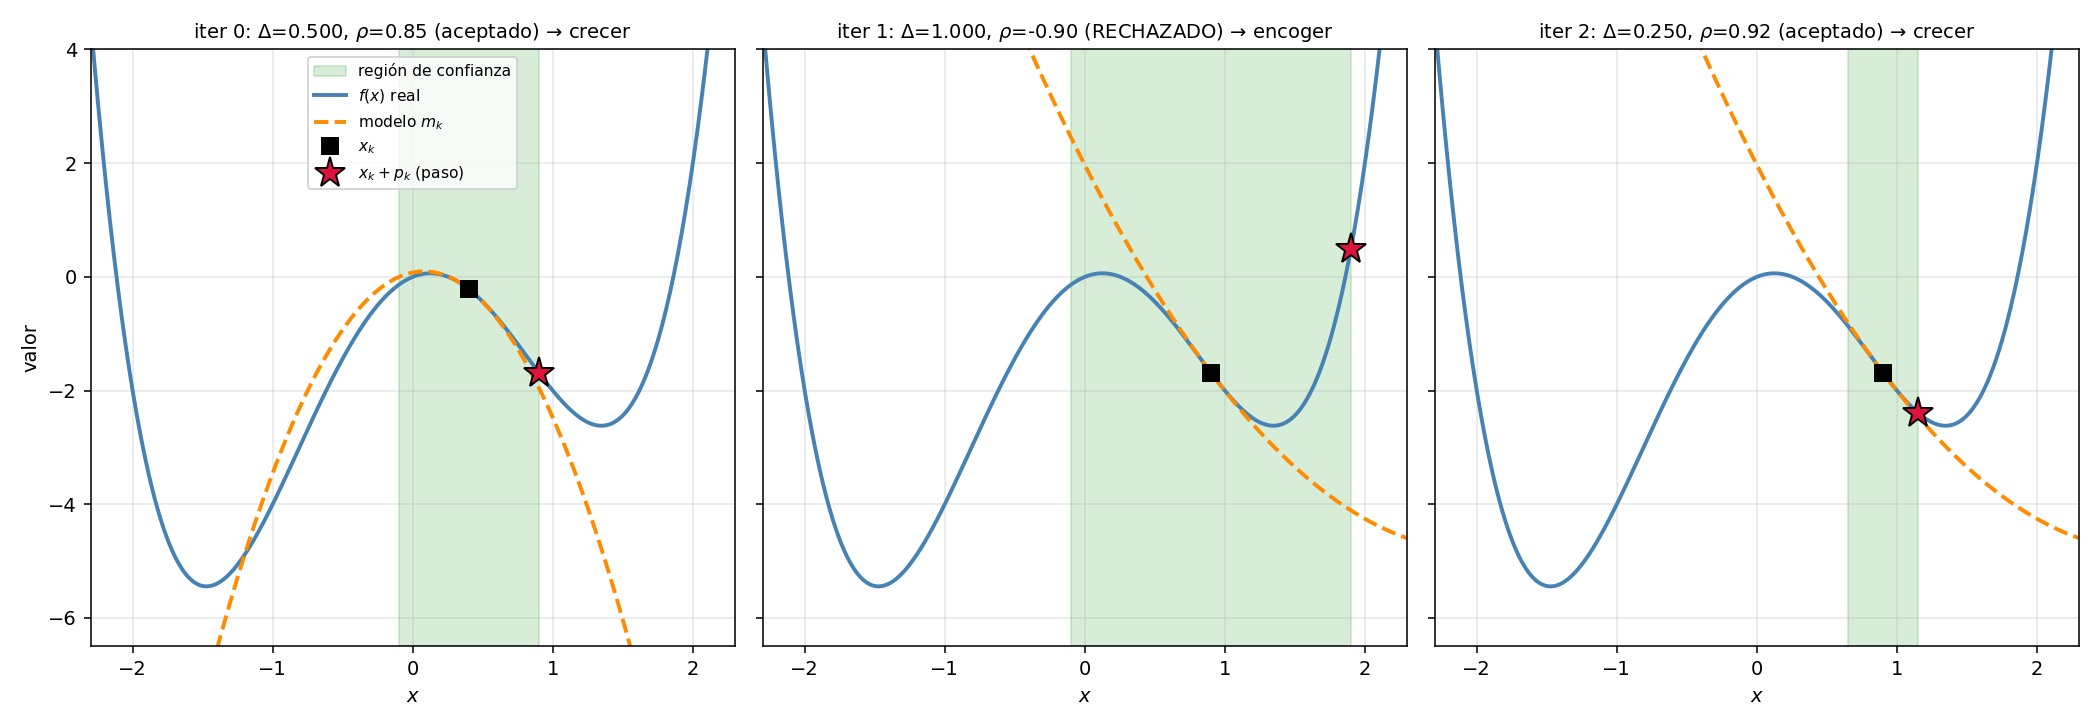
\includegraphics[width=\textwidth]{figs/fig07b_tr1d_iteraciones_a.png}
\end{frame}

\begin{frame}{Ejemplo (cont.): cerca del m\'inimo, el modelo ya es fiel}
  \small
  Con $\Delta=0.5$ el m\'inimo de la par\'abola (tri\'angulo morado) \textbf{cabe} en la regi\'on: el paso es el de Newton completo y $\rho_k\approx1$.
  \vspace{0.2cm}
  \centering
  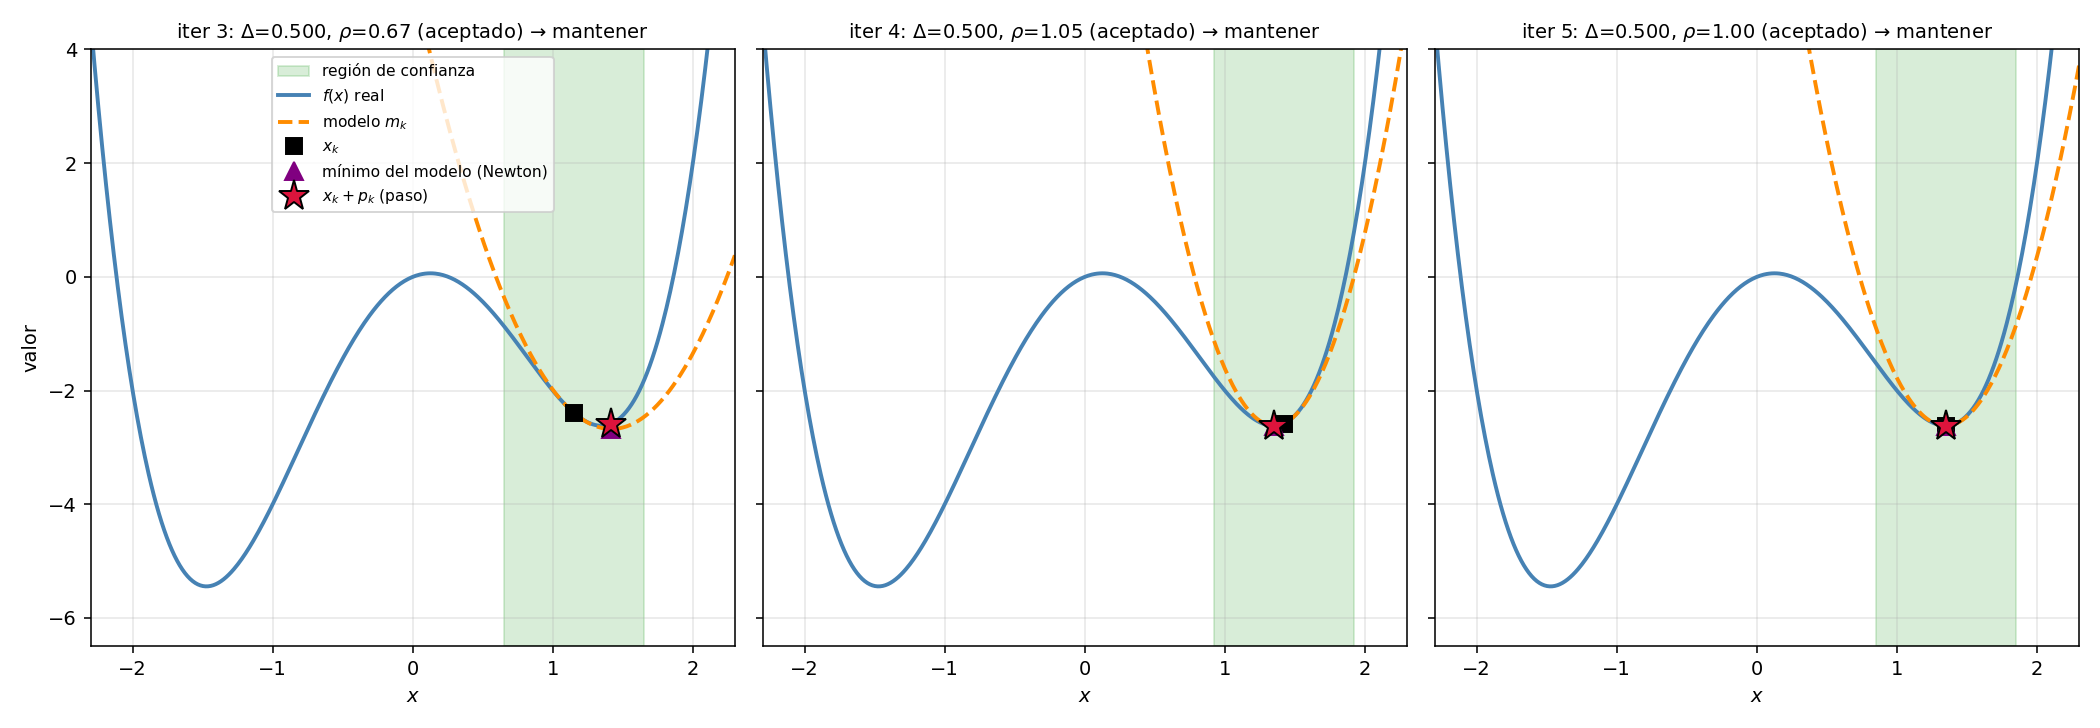
\includegraphics[width=\textwidth]{figs/fig07b_tr1d_iteraciones_b.png}
\end{frame}

\begin{frame}{Lectura iteraci\'on por iteraci\'on}
  \footnotesize
  \begin{tabular}{clccrl}
    \toprule
    $k$ & $x_k$ & $f''(x_k)$ & $\Delta_k$ & $\rho_k$ & qu\'e ocurre \\
    \midrule
    0 & 0.4000 & $-6.08$ & 0.500 & 0.85 & curvatura $<0$: va al borde; acepta; \textbf{crece} \\
    1 & 0.9000 & $1.72$  & 1.000 & $-0.90$ & Newton recortado; $f$ \textbf{sube}: \textbf{rechaza} y encoge \\
    2 & 0.9000 & $1.72$  & 0.250 & 0.92 & mismo $x_k$, radio menor; acepta; crece \\
    3 & 1.1500 & $7.87$  & 0.500 & 0.67 & Newton cabe en la regi\'on; acepta \\
    4 & 1.4189 & $16.16$ & 0.500 & 1.05 & Newton; acepta \\
    5 & 1.3524 & $13.95$ & 0.500 & 1.00 & Newton; acepta \\
    6 & 1.3470 & $13.77$ & 0.500 & 1.00 & Newton; $|f'|<10^{-6}$, termina \\
    \bottomrule
  \end{tabular}
  \vspace{0.3cm}
  \begin{itemize}
    \small
    \item \textbf{Iter.\ 1}: con $\Delta=1$ el modelo promet\'ia bajar mucho, pero $f$ sube ($\rho<0$). Al achicar la regi\'on a $0.25$ el modelo vuelve a ser fiel.
    \item \textbf{Cerca del m\'inimo} el modelo es casi exacto ($\rho\approx1$), el radio ya no estorba y se recupera la convergencia r\'apida de Newton.
  \end{itemize}
\end{frame}

\begin{frame}{Radio $\Delta_k$ y ratio $\rho_k$ a lo largo de las iteraciones}
  \centering
  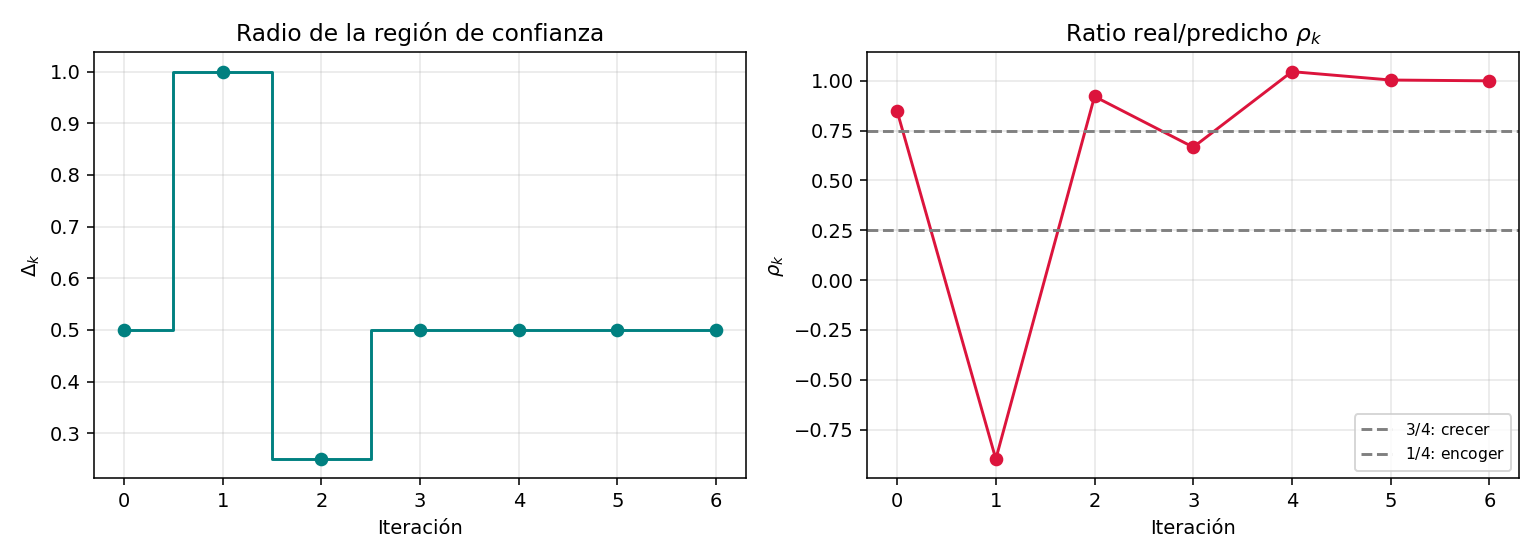
\includegraphics[width=0.92\textwidth]{figs/fig07b_tr1d_radio_rho.png}
  \vspace{0.1cm}
  \small
  \begin{itemize}
    \item Trust region 1D (manual): \textbf{7} iteraciones, $x^\star\approx1.34699741$, $f^\star\approx-2.6186$.
    \item \texttt{scipy trust-exact}: mismo m\'inimo en 4 iteraciones (par\'ametros distintos: radio inicial, umbrales de aceptaci\'on y resoluci\'on del subproblema); el n\'umero exacto depende de esas elecciones.
  \end{itemize}
\end{frame}

\begin{frame}{Los dos candidatos que combina dogleg}
  \small
  \begin{block}{Paso de Cauchy $p_C$}
    El minimizador de $m_k$ a lo largo de la direcci\'on de m\'aximo descenso $-\grad f(x_k)$, restringido a la bola:
    \[ p_C = -\frac{\grad f_k^T \grad f_k}{\grad f_k^T H_k \grad f_k}\, \grad f_k \quad \text{(truncado a la frontera si se sale de } \Delta_k) \]
    Barato, siempre disponible (incluso si $H_k$ no es definida positiva), pero \textbf{conservador}: es esencialmente un paso de descenso de gradiente.
  \end{block}
  \begin{block}{Paso de Newton $p_N$}
    \[ p_N = -H_k^{-1}\, \grad f_k \]
    El minimizador \textbf{exacto} de $m_k$ sin restricci\'on de radio. Ideal cuando $H_k$ es definida positiva y $\Delta_k$ es suficientemente grande --- pero puede salirse de la regi\'on, o no ser descenso si $H_k$ no es definida positiva.
  \end{block}
\end{frame}

\begin{frame}{?`De d\'onde sale la direcci\'on de Cauchy?}
  El gradiente del modelo cuadr\'atico respecto a $p$ es
  \[ \grad_p m_k(p) = \grad f(x_k) + H_k\, p \]
  Evaluado en $p=0$ (el punto de partida $x_k$ mismo, donde el t\'ermino cuadr\'atico se anula):
  \[ \grad_p m_k(0) = \grad f(x_k) \]
  \begin{alertblock}{Por eso la direcci\'on de Cauchy es $-\grad f(x_k)$}
    La direcci\'on de m\'aximo descenso \textbf{del modelo cuadr\'atico}, evaluada en el punto de partida, coincide exactamente con $-\grad f(x_k)$. No es una casualidad ni una simplificaci\'on: es consecuencia directa de que $m_k$ y $f$ comparten el mismo gradiente en $p=0$ (as\'i se construye el modelo de Taylor).
  \end{alertblock}
\end{frame}

\begin{frame}{Cuidado: minimizar \emph{sobre una recta} no es minimizar el modelo completo}
  El paso de Cauchy se obtiene en dos etapas:
  \begin{enumerate}
    \item Fijar la direcci\'on $d=-\grad f(x_k)$ (la de m\'aximo descenso de $m_k$ en $p=0$).
    \item Minimizar $m_k$ \textbf{restringido a esa recta}: $\displaystyle\min_{\alpha\geq0} m_k(\alpha\, d)$.
  \end{enumerate}
  \begin{alertblock}{Esto NO es lo mismo que minimizar $m_k$ sobre todo $\mathbb{R}^n$}
    Si en cambio se minimiza $m_k(p)$ dejando que \textbf{direcci\'on y magnitud} se ajusten libremente seg\'un la curvatura $H_k$, se llega al paso de \textbf{Newton}, $p_N=-H_k^{-1}\grad f_k$ --- que en general \textbf{no} es paralelo a $-\grad f_k$.
  \end{alertblock}
  \centering
  \small
  Excepci\'on: si $H_k=cI$ (curvatura isotr\'opica), $p_N=-\tfrac1c\grad f_k$ s\'i es paralelo a $p_C$, y el dogleg colapsa a un segmento recto.
\end{frame}

\begin{frame}{?`Qu\'e pasa si $H_k$ no es definida positiva?}
  \small
  \begin{block}{Caso $H_k$ definida positiva}
    $\grad f_k^T H_k \grad f_k > 0$: la par\'abola $m_k(\alpha\,(-\grad f_k))$ abre hacia arriba, $\alpha_C$ es un m\'inimo genuino y bien definido.
  \end{block}
  \begin{block}{Caso $H_k$ NO definida positiva ($\grad f_k^T H_k \grad f_k \leq 0$)}
    La restricci\'on de $m_k$ a la recta $-\grad f_k$ es c\'oncava o lineal: \textbf{no tiene m\'inimo finito}. Regla: ir hasta el borde de la regi\'on de confianza,
    \[ p_C = -\Delta_k\, \frac{\grad f_k}{\|\grad f_k\|} \]
  \end{block}
  \begin{alertblock}{Qu\'e significa para el dogleg}
    El paso de Cauchy \textbf{siempre existe}: no invierte $H_k$ y $-\grad f_k$ siempre es direcci\'on de descenso. El paso de Newton, en cambio, solo tiene sentido con $H_k$ definida positiva; si no lo es, se usa \textbf{solo Cauchy} (o se cambia el solver del subproblema). Newton amortiguado, por su parte, necesita una salvaguarda externa.
  \end{alertblock}
\end{frame}

\begin{frame}{La trayectoria dogleg}
  Se define la poligonal $p(\tau)$, $\tau\in[0,2]$:
  \[
  p(\tau) = \begin{cases}
    \tau\, p_C, & 0 \leq \tau \leq 1 \\
    p_C + (\tau-1)(p_N - p_C), & 1 \leq \tau \leq 2
  \end{cases}
  \]
  Es decir: primero va del origen a $p_C$ en l\'inea recta, y luego de $p_C$ a $p_N$.

  \begin{alertblock}{Propiedad clave (Nocedal \& Wright, Lema 4.2)}
    $\|p(\tau)\|$ crece \textbf{mon\'otonamente} con $\tau$. Por lo tanto hay, a lo sumo, un \'unico $\tau^\star$ en el segundo tramo donde la poligonal cruza la frontera $\|p\|=\Delta_k$ --- y ese cruce se puede encontrar resolviendo una simple ecuaci\'on cuadr\'atica en $\tau$.
  \end{alertblock}
\end{frame}

\begin{frame}{Regla de selecci\'on del paso dogleg}
  Dado el radio actual $\Delta_k$:
  \begin{enumerate}
    \item \textbf{Si $\|p_N\| \leq \Delta_k$}: usar el paso de Newton completo, $p_k=p_N$ (cabe en la regi\'on; es el mejor paso posible).
    \item \textbf{Si $\|p_C\| \geq \Delta_k$}: usar $p_k = \Delta_k\, p_C/\|p_C\|$ (ni el paso de Cauchy cabe; truncar a lo largo de $-\grad f_k$).
    \item \textbf{En otro caso} ($\|p_C\| < \Delta_k < \|p_N\|$): el paso cruza el segundo tramo. Resolver
    \[ \|p_C + \tau(p_N-p_C)\|^2 = \Delta_k^2, \qquad \tau\in[0,1] \]
    (ecuaci\'on cuadr\'atica en $\tau$, se toma la ra\'iz positiva) y usar $p_k = p_C + \tau(p_N-p_C)$.
  \end{enumerate}
\end{frame}

\begin{frame}{Esquema: c\'omo intersecta la poligonal la frontera}
  \centering
  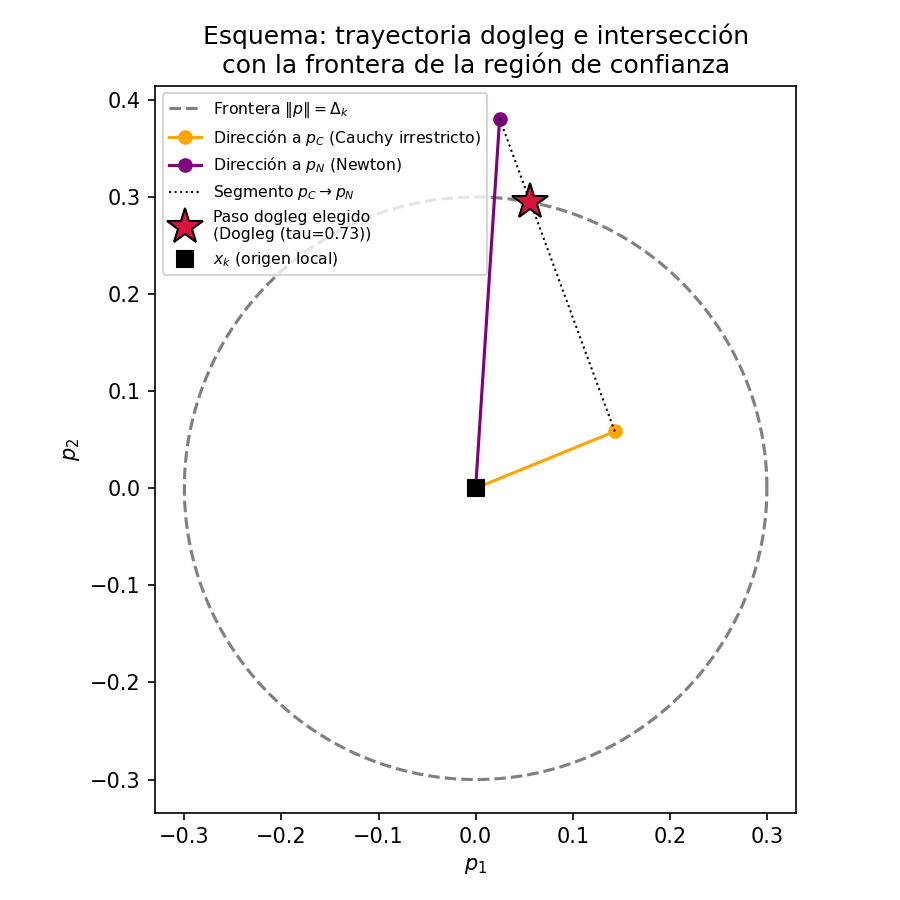
\includegraphics[height=0.82\textheight]{figs/fig07_dogleg_esquema.png}
\end{frame}

\begin{frame}{C\'omo se ajusta el radio $\Delta_k$ en cada iteraci\'on}
  Se mide qu\'e tan bien predijo el modelo cuadr\'atico la reducci\'on \textbf{real} de $f$:
  \[
  \rho_k = \frac{f(x_k) - f(x_k+p_k)}{m_k(0) - m_k(p_k)} = \frac{\text{reducci\'on real}}{\text{reducci\'on predicha por el modelo}}
  \]
  \begin{block}{Regla de actualizaci\'on}
    \begin{itemize}
      \item $\rho_k < 1/4$ (predicci\'on mala) $\Rightarrow$ \textbf{encoger}: $\Delta_{k+1}=0.25\,\Delta_k$.
      \item $\rho_k > 3/4$ \textbf{y} $\|p_k\|=\Delta_k$ (el paso us\'o todo el radio disponible y el modelo fue fiel) $\Rightarrow$ \textbf{crecer}: $\Delta_{k+1}=\min(2\Delta_k,\, \Delta_{\max})$.
      \item En otro caso $\Rightarrow$ mantener $\Delta_{k+1}=\Delta_k$.
    \end{itemize}
  \end{block}
  \textbf{Aceptaci\'on del paso}: si $\rho_k>0$, se acepta $x_{k+1}=x_k+p_k$; si no, se rechaza ($x_{k+1}=x_k$) y solo se encoge la regi\'on para reintentar.
\end{frame}

\begin{frame}[fragile]{C\'odigo: paso dogleg (los 3 casos)}
\begin{lstlisting}
if np.linalg.norm(pN) <= Delta:
    p = pN                                    # caso 1: Newton completo
elif np.linalg.norm(pC) >= Delta:
    p = Delta / np.linalg.norm(pC) * pC        # caso 2: Cauchy truncado
else:
    d = pN - pC
    a = d @ d; b = 2*pC @ d; c = pC @ pC - Delta**2
    tau = (-b + np.sqrt(b**2 - 4*a*c)) / (2*a)  # caso 3: interseccion
    p = pC + tau * d
\end{lstlisting}
\end{frame}

\begin{frame}[fragile]{C\'odigo: actualizaci\'on del radio (ratio $\rho_k$)}
\begin{lstlisting}
pred = -(g @ p + 0.5 * p @ H @ p)          # m(0) - m(p)
actual = f(x) - f(x + p)
rho = actual / pred if pred > 1e-14 else -1.0

if rho > 0:
    x = x + p                              # aceptar paso
if rho < 0.25:
    Delta = 0.25 * Delta                   # encoger
elif rho > 0.75 and np.isclose(np.linalg.norm(p), Delta):
    Delta = min(2 * Delta, Delta_max)      # crecer
\end{lstlisting}
\end{frame}

\begin{frame}{Trayectoria: dogleg en Rosenbrock}
  \centering
  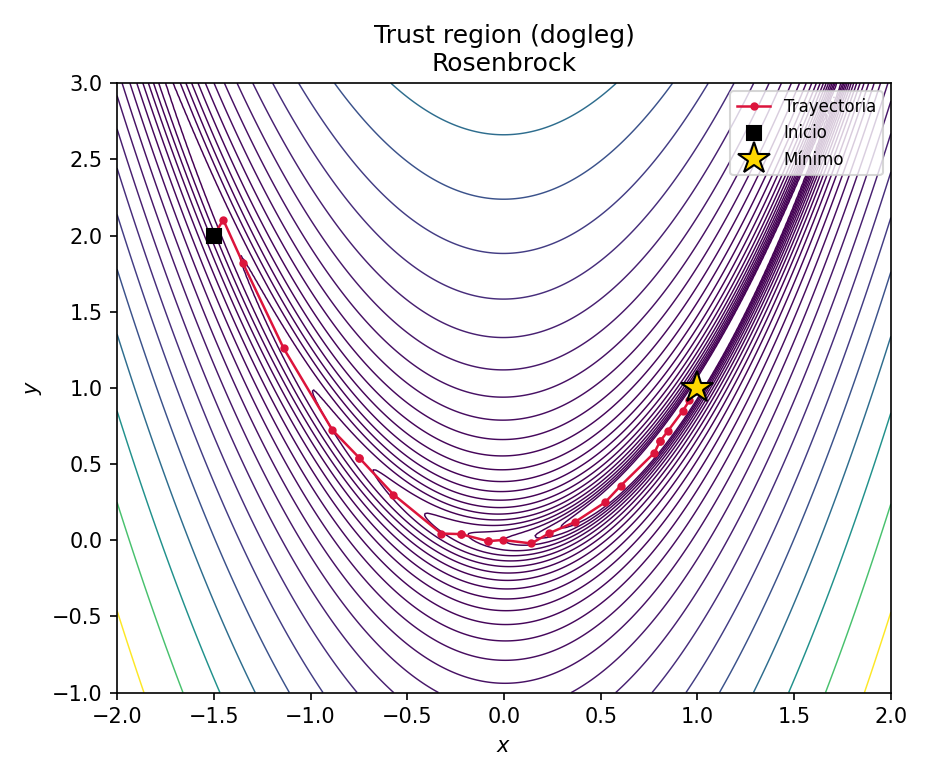
\includegraphics[height=0.82\textheight]{figs/fig07_dogleg_rosenbrock.png}
\end{frame}

\begin{frame}{Evoluci\'on del radio de la regi\'on de confianza}
  \centering
  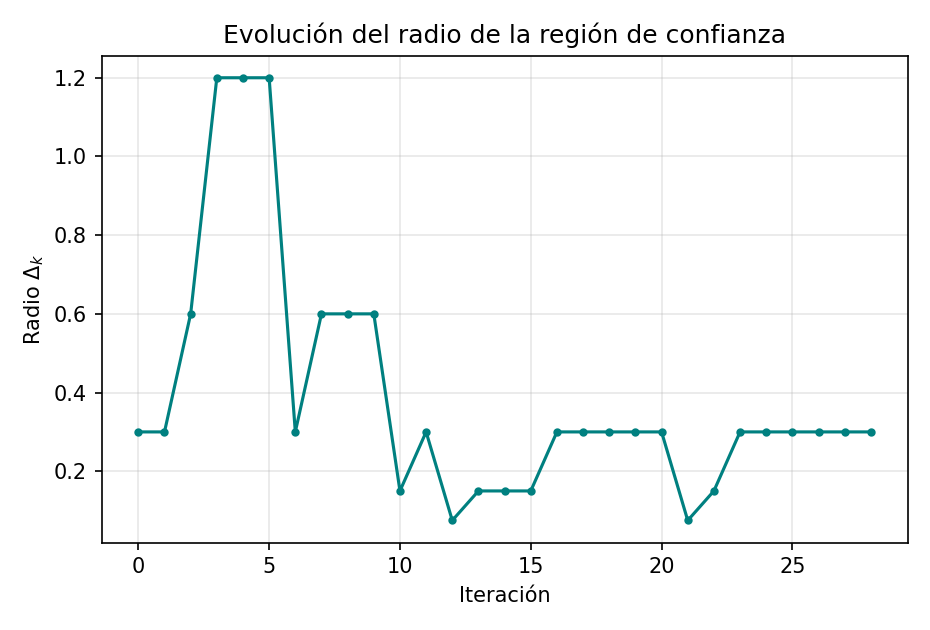
\includegraphics[height=0.82\textheight]{figs/fig07_dogleg_radio.png}
\end{frame}

\begin{frame}{Resultados}
  \begin{itemize}
    \item Trust region dogleg (manual): \textbf{29} iteraciones, mezcla de pasos ``Newton'' (cuando $p_N$ cabe) y ``Dogleg'' (cuando cruza la frontera) --- ver primeras 15 iteraciones: \texttt{[Newton, Dogleg($\tau$=0.06), Dogleg($\tau$=0.13), Newton, Newton, Newton, Dogleg($\tau$=0.46), ...]}
    \item Radio $\Delta_k$: parte en $0.3$, llega a oscilar entre $0.075$ y $1.2$ seg\'un qu\'e tan bien predice el modelo local.
    \item \texttt{scipy.optimize.minimize(method=`dogleg')}: 24 iteraciones --- resultado muy similar, confirmando la implementaci\'on manual.
  \end{itemize}
  \begin{alertblock}{Por qu\'e importa}
    Trust region es \textbf{robusto} porque el paso de Cauchy siempre existe y reduce el modelo: si $H_k$ no es definida positiva se recurre a \'el (una l\'inea en el c\'odigo), sin la salvaguarda ad-hoc de Newton amortiguado.
  \end{alertblock}
\end{frame}
% ============================================================
\section{Levenberg-Marquardt}
% ============================================================

\begin{frame}{M\'inimos cuadrados no lineales}
  Un caso muy frecuente en ingenier\'ia: ajustar un modelo a datos minimizando
  \[ f(x) = \tfrac12\|r(x)\|^2 = \tfrac12\sum_{i=1}^m r_i(x)^2, \qquad r:\mathbb{R}^n\to\mathbb{R}^m \]
  donde $r_i(x)$ es el residuo (diferencia modelo--dato) del punto $i$.

  Para este $f$ en particular:
  \[ \grad f(x) = J(x)^T r(x), \qquad H(x) = J(x)^T J(x) + \underbrace{\sum_i r_i(x)\, \grad^2 r_i(x)}_{\text{se descarta}} \]
  \textbf{Aproximaci\'on de Gauss-Newton}: $H(x) \approx J(x)^T J(x)$ (exacta si $r$ es lineal, o si los residuos son peque\~nos cerca del \'optimo).
\end{frame}

\begin{frame}{El paso de Levenberg-Marquardt}
  \begin{block}{Sistema regularizado}
    \[ \big(J^T J + \lambda I\big)\, p = -J^T r \]
  \end{block}
  \begin{itemize}
    \item $\lambda \to 0$: $p$ tiende al paso de \textbf{Gauss-Newton} (casi-Newton, r\'apido si los residuos son peque\~nos).
    \item $\lambda \to \infty$: $p \to -\tfrac1\lambda J^T r$, un paso de \textbf{descenso de gradiente} muy corto (lento pero robusto).
  \end{itemize}
  \begin{alertblock}{Relaci\'on con trust region}
    $\lambda$ juega el mismo papel que $1/\Delta_k$ en dogleg: se ajusta seg\'un el mismo ratio $\rho_k$ de reducci\'on real/predicha. Si el paso mejora $f$: aceptar y \textbf{bajar} $\lambda$ (confiar m\'as en Gauss-Newton). Si empeora: rechazar y \textbf{subir} $\lambda$ (retroceder hacia gradiente). LM es, en esencia, un trust region impl\'icito especializado a m\'inimos cuadrados.
  \end{alertblock}
\end{frame}

\begin{frame}{Ejemplo: ajuste de un decaimiento exponencial}
  Datos sint\'eticos ruidosos generados con $y(t) = A\,e^{-kt} + b$, $(A,k,b)=(5,\,0.7,\,1)$, ruido gaussiano $\sigma=0.15$. Estimaci\'on inicial deliberadamente mala: $(A_0,k_0,b_0)=(1,\,0.1,\,0)$.
  \[
  r_i(A,k,b) = A\,e^{-k t_i} + b - y_i, \qquad i=1,\dots,40
  \]
  Jacobiano anal\'itico: $\partial r_i/\partial A = e^{-kt_i}$, $\;\partial r_i/\partial k = -A t_i e^{-kt_i}$, $\;\partial r_i/\partial b = 1$.

  \texttt{scipy.optimize.curve\_fit} y \texttt{scipy.optimize.least\_squares(method=`lm')} usan Levenberg-Marquardt por defecto para este tipo exacto de problema.
\end{frame}

\begin{frame}[fragile]{C\'odigo: n\'ucleo de Levenberg-Marquardt}
\begin{lstlisting}
JTJ = J.T @ J;  g = J.T @ r;  f_cur = 0.5 * r @ r
for _ in range(30):
    A_lm = JTJ + lam * np.eye(n)
    p = np.linalg.solve(A_lm, -g)
    f_new = 0.5 * np.sum(res_fun(theta + p)**2)
    pred = -(g @ p + 0.5 * p @ JTJ @ p)
    rho = (f_cur - f_new) / pred if pred > 1e-14 else -1.0
    if rho > 0:
        theta = theta + p;  lam = max(lam*0.5, 1e-12);  break
    else:
        lam *= 3.0
\end{lstlisting}
\end{frame}

\begin{frame}{Trayectoria en el espacio de par\'ametros $(A,k)$}
  \centering
  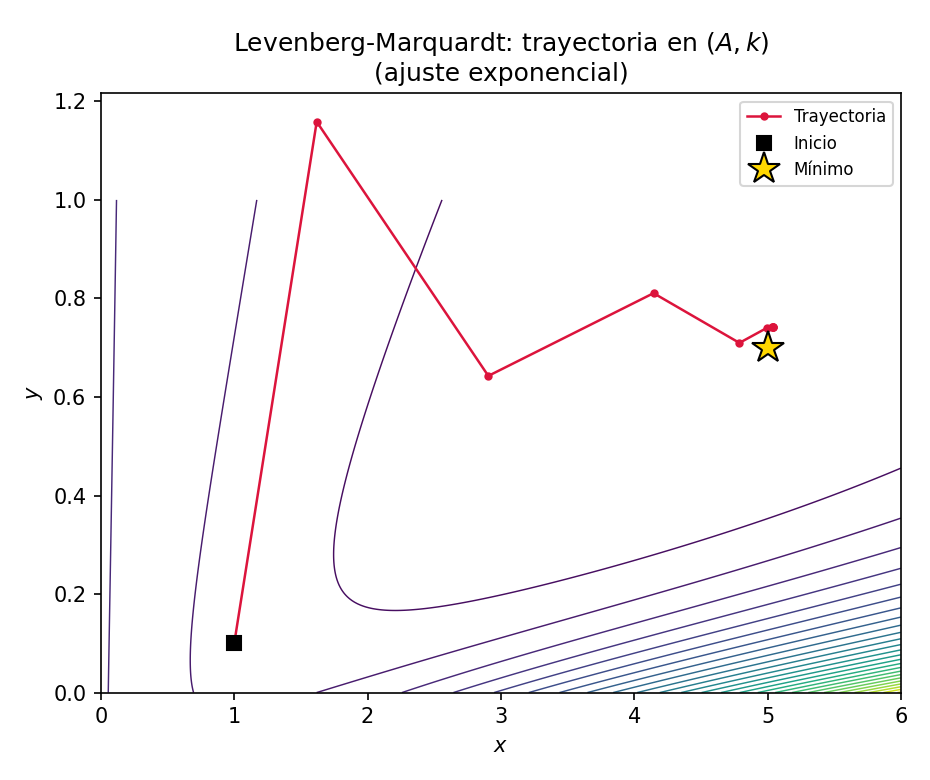
\includegraphics[height=0.82\textheight]{figs/fig08_lm_trayectoria_Ak.png}
\end{frame}

\begin{frame}{Ajuste final y convergencia}
  \begin{columns}[T]
    \begin{column}{0.5\textwidth}
      \centering
      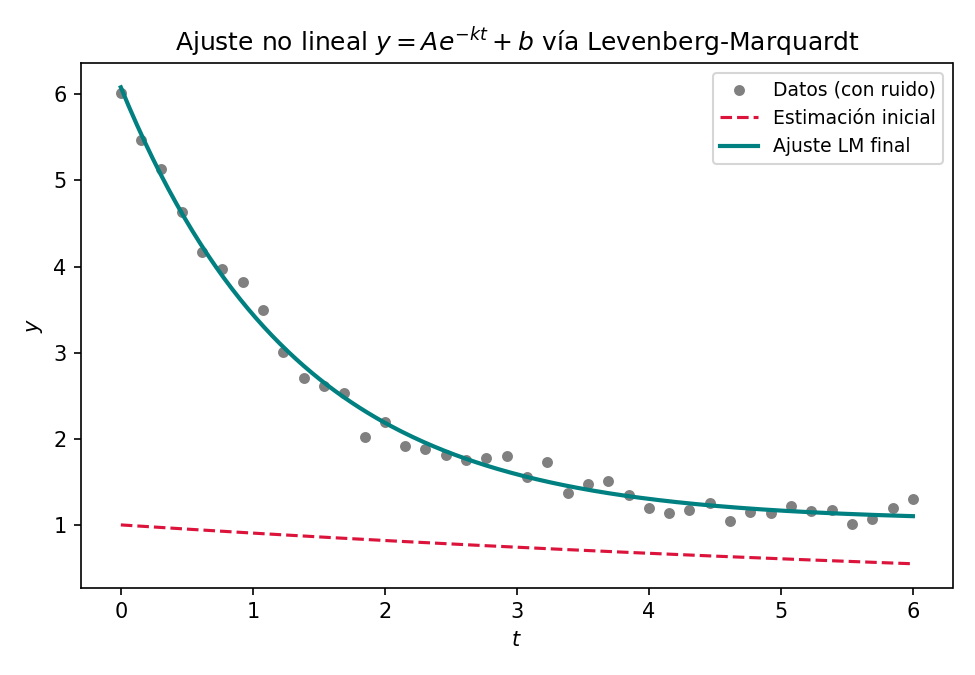
\includegraphics[width=\textwidth]{figs/fig08_lm_ajuste.png}
    \end{column}
    \begin{column}{0.48\textwidth}
      \centering
      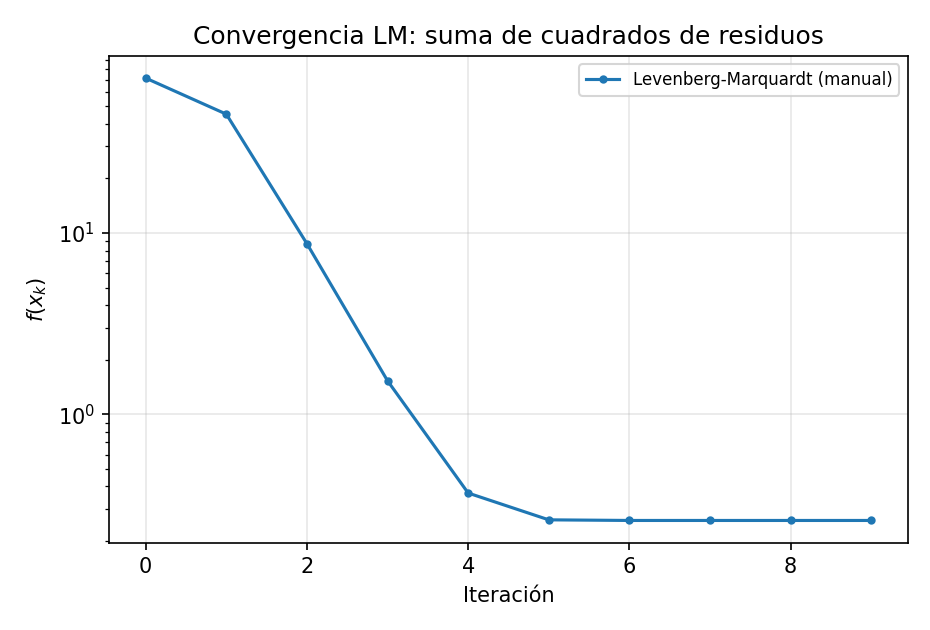
\includegraphics[width=\textwidth]{figs/fig08_lm_convergencia.png}
    \end{column}
  \end{columns}
  \vspace{0.2cm}
  \begin{itemize}
    \small
    \item LM manual: \textbf{10} iteraciones, $(A,k,b)_{\text{final}} = (5.038,\,0.741,\,1.042)$.
    \item \texttt{scipy least\_squares(lm)}: 10 evaluaciones, resultado \textbf{id\'entico} hasta 5 cifras.
    \item Los valores no coinciden exactamente con $(5,\,0.7,\,1)$ porque el ajuste es sobre datos \textbf{ruidosos} --- eso es exactamente lo esperado en un problema de m\'inimos cuadrados.
  \end{itemize}
\end{frame}

% ============================================================
\section{Gradiente estoc\'astico (SGD)}
% ============================================================

\begin{frame}{Motivaci\'on: cuando $N$ es enorme}
  Muchos problemas (t\'ipicamente en aprendizaje autom\'atico, pero tambi\'en en ajuste de modelos con much\'isimos datos) tienen la forma
  \[ f(x) = \frac1N \sum_{i=1}^N f_i(x) \]
  El gradiente completo $\grad f(x) = \tfrac1N\sum_i \grad f_i(x)$ cuesta $O(N)$ \textbf{por iteraci\'on}. Si $N$ son millones de datos, eso es prohibitivo.

  \begin{block}{Idea: gradiente estoc\'astico (SGD)}
    Reemplazar el gradiente completo por un \textbf{estimador ruidoso pero barato}, calculado sobre un subconjunto (\emph{minibatch}) $B_k$ de tama\~no $b\ll N$ elegido al azar:
    \[ x_{k+1} = x_k - \alpha_k \cdot \frac1b \sum_{i\in B_k} \grad f_i(x_k) \]
  \end{block}
\end{frame}

\begin{frame}{Paso constante vs. paso decreciente}
  Ejemplo: regresi\'on lineal por m\'inimos cuadrados, $N=500$ datos, minibatches de tama\~no $b=10$.
  \begin{itemize}
    \item \textbf{Paso constante} $\alpha=0.05$: NO converge al \'optimo exacto --- la trayectoria entra en una ``nube'' de ruido alrededor de \'el (la varianza del estimador de gradiente no desaparece).
    \item \textbf{Paso decreciente} $\alpha_k = \alpha_0/(1+k)$: s\'i converge, porque el ruido se apaga junto con el paso --- a costa de avanzar m\'as lento al final.
  \end{itemize}
\end{frame}

\begin{frame}{Trayectorias: paso constante vs. decreciente vs. batch}
  \centering
  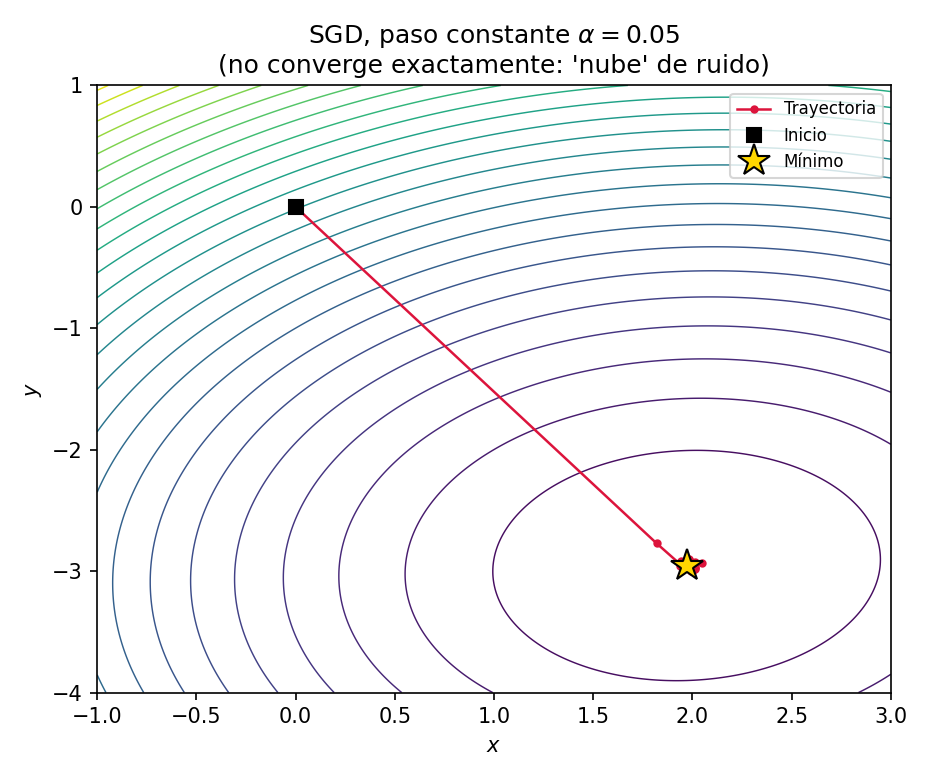
\includegraphics[width=0.32\textwidth]{figs/fig09_sgd_paso_constante.png}%
  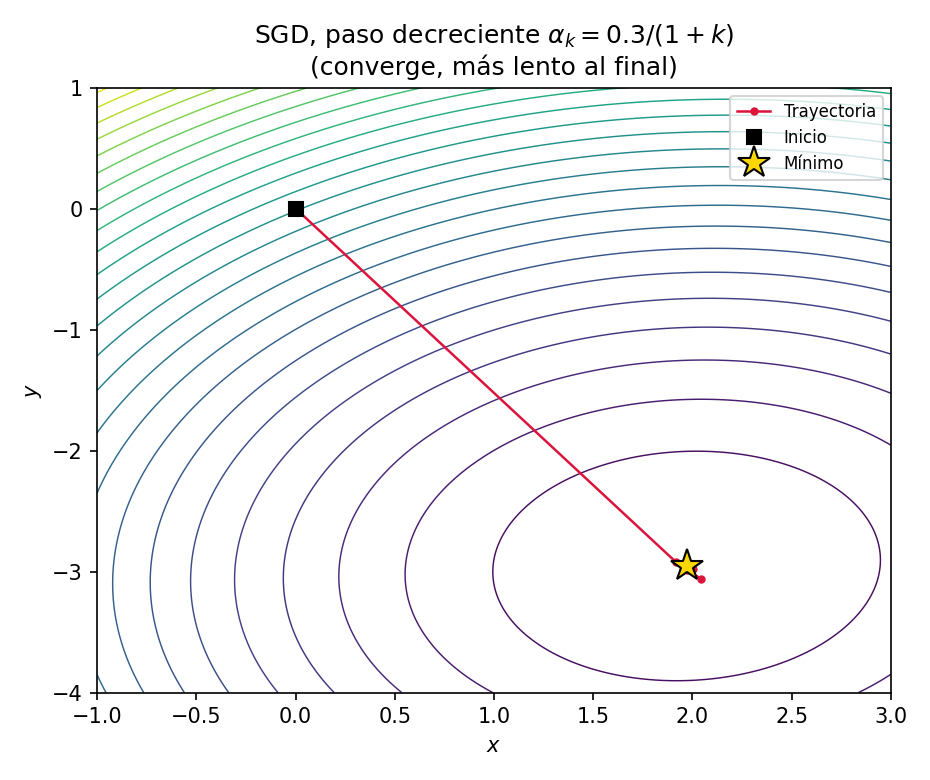
\includegraphics[width=0.32\textwidth]{figs/fig09_sgd_paso_decreciente.png}%
  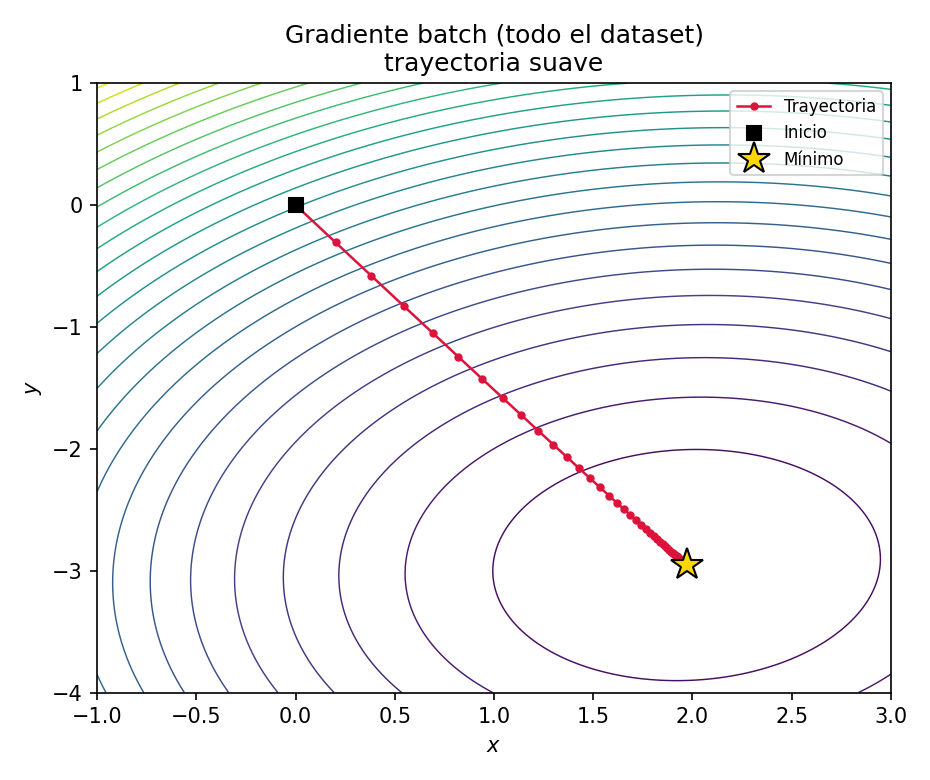
\includegraphics[width=0.32\textwidth]{figs/fig09_batch_gd.png}
  \begin{itemize}
    \small
    \item $\|w-w^\star\|$ final: paso constante $0.0136$, paso decreciente $\mathbf{0.0023}$, batch $0.0454$ (con el mismo n\'umero de \'epocas y un $\alpha$ razonable para cada uno).
  \end{itemize}
\end{frame}

\begin{frame}{P\'erdida por \'epoca: SGD vs. gradiente batch}
  \centering
  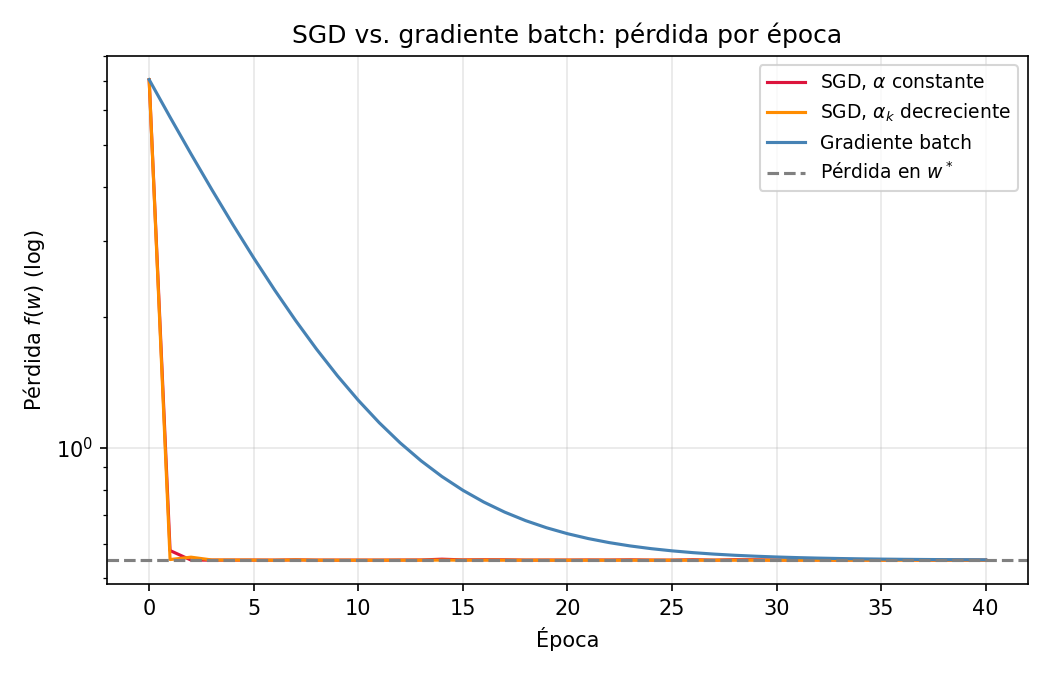
\includegraphics[height=0.78\textheight]{figs/fig09_sgd_vs_batch_perdida.png}
\end{frame}

\begin{frame}{Por qu\'e SGD baja m\'as r\'apido \emph{por \'epoca}}
  \begin{itemize}
    \item En una \'epoca, SGD recorre los $N=500$ datos --- igual que un paso de gradiente batch --- pero los agrupa en minibatches de $b=10$ y \textbf{actualiza $w$ 50 veces} (una por minibatch), no una sola vez.
    \item Por eso, a igual n\'umero de \'epocas (mismo costo total de evaluaciones de $\grad f_i$), SGD hace muchas m\'as actualizaciones de $x$ y baja la p\'erdida mucho m\'as r\'apido al principio.
    \item El precio: cada actualizaci\'on individual es ruidosa (basada en solo 10 datos), de ah\'i la ``nube'' alrededor del \'optimo con paso constante.
  \end{itemize}
  \begin{alertblock}{Conexi\'on con el resto de la clase}
    SGD es descenso de gradiente (script 1) con un $\grad f$ \textbf{aproximado}. Todo lo visto sobre el tama\~no de paso sigue aplicando --- salvo que ahora, adem\'as del tama\~no, importa el \textbf{ruido} del estimador.
  \end{alertblock}
\end{frame}
% ============================================================
\section{S\'intesis}
% ============================================================

\begin{frame}{Tabla comparativa}
  \footnotesize
  \begin{tabular}{lccc}
    \toprule
    M\'etodo & Usa & Estrategia & Convergencia \\
    \midrule
    Grad.\ (paso fijo) & $\grad f$ & --- & lineal, puede divergir \\
    Grad.\ + Armijo & $\grad f$ & line search & lineal, robusta \\
    Powell & solo $f$ & line search (conjugadas) & superlineal \\
    Newton & $\grad f, H$ & line search / amortiguado & cuadr\'atica (local) \\
    Quasi-Newton (BFGS) & $\grad f$ & line search & superlineal \\
    Trust region (dogleg) & $\grad f, H$ & trust region & superlin./cuadr\'atica \\
    Levenberg-Marquardt & $J$ (m\'in.\ cuadr.) & trust region impl\'icito & superlineal \\
    SGD & $\grad f_i$ (ruidoso) & line search impl\'icito & sublineal (ruidosa) \\
    \bottomrule
  \end{tabular}
  \vspace{0.4cm}
  \begin{itemize}
    \small
    \item \textbf{Sin derivadas} $\to$ Powell. \textbf{Con gradiente, sin Hessiana} $\to$ BFGS. \textbf{Con Hessiana} $\to$ Newton o dogleg (dogleg m\'as robusto si $H$ no siempre es definida positiva). \textbf{M\'inimos cuadrados} $\to$ Levenberg-Marquardt. \textbf{Datos masivos} $\to$ SGD.
  \end{itemize}
\end{frame}

\begin{frame}{Lo que tienen en com\'un}
  \begin{itemize}
    \item Todos generan una sucesi\'on $x_{k+1}=x_k+\alpha_k d_k$ (o su equivalente en trust region, $x_{k+1}=x_k+p_k$).
    \item Todos necesitan alg\'un mecanismo de \textbf{control de paso} (line search o radio de confianza) para garantizar que efectivamente se reduce $f$ --- sin \'el, como vimos en el paso fijo, se puede divergir.
    \item La \textbf{curvatura} (Hessiana exacta o aproximada) es lo que separa los m\'etodos lentos (descenso de gradiente, decenas de miles de iteraciones en valles curvos) de los r\'apidos (Newton/quasi-Newton/dogleg, decenas de iteraciones).
  \end{itemize}
\end{frame}

\begin{frame}{Roadmap del curso}
  \begin{itemize}
    \item \textbf{Clases 1--3}: fundamentos anal\'iticos, b\'usqueda 1D/multidimensional, metaheur\'isticas estoc\'asticas.
    \item \textbf{Clase 4 (hoy)}: m\'etodos basados en direcci\'on de b\'usqueda --- gradiente, Newton, quasi-Newton, trust region, LM, SGD.
    \item \textbf{Pr\'oximos pasos posibles}: programaci\'on lineal (simplex, punto interior); programaci\'on no lineal con restricciones (SQP, m\'etodos de penalizaci\'on y de barrera, combinando las ideas de hoy con las condiciones KKT de la Clase 1).
  \end{itemize}
\end{frame}

\begin{frame}{Ejercicios propuestos}
  \small
  \begin{enumerate}
    \item Repetir el descenso de gradiente de paso fijo variando $\kappa$ (n\'umero de condici\'on) y graficar el n\'umero de iteraciones necesarias vs. $\kappa$.
    \item Implementar la condici\'on de curvatura de Wolfe (adem\'as de Armijo) en el backtracking y comparar el n\'umero de iteraciones resultante en Rosenbrock.
    \item Modificar Powell para reiniciar peri\'odicamente a los ejes coordenados (cada $n$ ciclos) y comparar la robustez con la versi\'on original.
    \item Comparar Newton puro (sin amortiguar) vs. Newton amortiguado partiendo de un punto donde la Hessiana de Rosenbrock no es definida positiva; verificar en qu\'e iteraciones act\'ua la salvaguarda.
    \item Implementar el m\'etodo trust region con el subproblema resuelto exactamente (m\'etodo de Mor\'e-Sorensen) y comparar el n\'umero de iteraciones con dogleg.
    \item Extender el ejemplo de SGD a un tama\~no de minibatch variable ($b\in\{1,10,50,500\}$) y estudiar el trade-off entre ruido y velocidad de convergencia por \'epoca.
  \end{enumerate}
\end{frame}

\begin{frame}{Referencias}
  \footnotesize
  \begin{itemize}
    \item J. Nocedal, S. J. Wright, \emph{Numerical Optimization}, 2\textsuperscript{a} ed., Springer, 2006. (Cap.\ 3: line search; Cap.\ 4: trust region/dogleg; Cap.\ 6: quasi-Newton; Cap.\ 10: m\'inimos cuadrados no lineales.)
    \item S. Boyd, L. Vandenberghe, \emph{Convex Optimization}, Cambridge University Press, 2004.
    \item D. P. Bertsekas, \emph{Nonlinear Programming}, 3\textsuperscript{a} ed., Athena Scientific, 2016.
    \item K. Levenberg, ``A Method for the Solution of Certain Non-Linear Problems in Least Squares'', \emph{Quarterly of Applied Mathematics}, 1944.
    \item D. Marquardt, ``An Algorithm for Least-Squares Estimation of Nonlinear Parameters'', \emph{SIAM J. Appl. Math.}, 1963.
    \item M. J. D. Powell, ``An efficient method for finding the minimum of a function of several variables without calculating derivatives'', \emph{Computer Journal}, 1964.
    \item L. Bottou, F. E. Curtis, J. Nocedal, ``Optimization Methods for Large-Scale Machine Learning'', \emph{SIAM Review}, 2018. (SGD.)
  \end{itemize}
\end{frame}

\begin{frame}[standout]
  Fin de la Clase 4
\end{frame}

\end{document}
